\part{抽象代数}

\chapter{群}
\section{群}
\subsection{半群}
\begin{definition}\label{definition:抽象代数.半群的定义}
设\(G\)是非空集合,
\(\times\)是定义在\(G\)上的一个二元代数运算.
% \hyperref[definition:集合论.二元代数运算]{二元代数运算}蕴含了“集合\(G\)对\(\times\)运算封闭”这个条件,因此省略
如果\(\times\)满足结合律,即\begin{equation*}
	(\forall a,b,c \in G)
	[(a \times b) \times c = a \times (b \times c)],
\end{equation*}
那么称“定义了\(\times\)运算的\(G\)集\(\opair{G,\times}\)是一个\DefineConcept{半群}(semigroup)”,
或称“集合\(G\)对于\(\times\)运算成半群”.
\end{definition}

由\cref{equation:集合论.自然数加法结合律,equation:集合论.自然数乘法结合律}
以及\cref{equation:集合论.整数加法结合律,equation:集合论.整数乘法结合律},
自然数集\(\omega\)、整数集\(\mathbb{Z}\)对于加法、乘法分别成半群,即\begin{equation*}
	\opair{\omega,+}, \qquad
	\opair{\omega,\times}, \qquad
	\opair{\mathbb{Z},+}, \qquad
	\opair{\mathbb{Z},\times}
\end{equation*}都是半群.

\subsection{单位元,幺半群}
下面我们给出左单位元、右单位元的定义,并证明左单位元、右单位元是同一的.
设\(G\)是非空集合,
\(\times\)是定义在\(G\)上的一个二元代数运算.
把满足\begin{equation*}
	e \in G
	\land
	(\forall a \in G)[e \times a = a]
\end{equation*}的元素\(e\)称为“\(\opair{G,\times}\)的\DefineConcept{左单位元}(left identity)”;
把满足\begin{equation*}
	o \in G
	\land
	(\forall a \in G)[a \times o = a]
\end{equation*}的元素\(o\)称为“\(\opair{G,\times}\)的\DefineConcept{右单位元}(right identity)”.

假设左单位元、右单位元都存在,
那么\begin{equation*}
	e = e \times o = o,
\end{equation*}
这就是说\(\opair{G,\times}\)的左单位元就是它的右单位元;
这时候我们把\(\opair{G,\times}\)的左单位元、右单位元合称为%
“\(\opair{G,\times}\)的\DefineConcept{单位元}(identity)”.

\begin{example}\label{example:抽象代数.单位元.例1}
我们可以构造一个对集\(G = \Set{ a, b }\),其中\(a \neq b\).
再定义:\begin{equation*}
	\times = \Set{
		\opair{\opair{a,b},b},
		\opair{\opair{b,a},a},
		\opair{\opair{a,a},a},
		\opair{\opair{b,b},b}
	}.
\end{equation*}
容易看出\(a,b\)都是\(G\)的左单位元.
由于\begin{align*}
	(a \times a) \times a = a = a \times (a \times a), \\
	(a \times a) \times b = b = a \times (a \times b), \\
	(a \times b) \times a = a = a \times (b \times a), \\
	(b \times a) \times a = a = b \times (a \times a), \\
	(a \times b) \times b = b = a \times (b \times b), \\
	(b \times a) \times b = b = b \times (a \times b), \\
	(b \times b) \times a = a = b \times (b \times a), \\
	(b \times b) \times b = b = b \times (b \times b),
\end{align*}
所以\(\times\)服从结合律.
综上所述,\(\opair{G,\times}\)是一个只有左逆元而没有右逆元的半群.
\end{example}

\begin{example}
我们可以把\cref{example:抽象代数.单位元.例1} 中定义的\(\times\)运算画成一个表格:
\begin{center}
\begin{tabular}{c|cc}
	\(\times\) & \(a\) & \(b\) \\ \hline
	\(a\) & \(a\) & \(b\) \\
	\(b\) & \(a\) & \(b\) \\
\end{tabular}
\end{center}
在阅读时,我们从\(\times\)算符下边任取一个元素,确定一行;
然后再从\(\times\)算符右边任取一个元素,确定一列;
行列相交之处的元素,就是上面我们取得的两个元素的运算结果.
例如,我们先取\(a\),这一行对过来的可能结果有\(a\)、\(b\)两个;
然后取\(b\),这一列对下去的可能结果只有重复的两个\(b\);
那么相交之处就是\(b\),也就是说\(a \times b = b\).
\end{example}

\begin{definition}\label{definition:抽象代数.幺半群的定义}
设\(\opair{G,\times}\)是半群.
如果\(G\)中存在单位元,即\begin{equation*}
	(\exists e \in G)(\forall a \in G)
	[e \times a = a \times e = a].
\end{equation*}
那么称“定义了\(\times\)运算的\(G\)集\(\opair{G,\times}\)是一个\DefineConcept{幺半群}(monoid)”,
或称“集合\(G\)对于\(\times\)运算成幺半群”.
\end{definition}

由于根据\cref{equation:集合论.自然数的加法.性质1,%
equation:集合论.自然数加法交换律,%
equation:集合论.自然数的乘法.性质1,%
equation:集合论.自然数乘法交换律,%
equation:集合论.任意整数加上零不变,%
equation:集合论.整数加法交换律,%
equation:集合论.任意整数乘上一不变,%
equation:集合论.整数乘法交换律},
\(0\)是自然数加法\(\opair{\omega,+}\)、整数加法\(\opair{\mathbb{Z},+}\)的单位元,
\(1\)是自然数乘法\(\opair{\omega,\times}\)、整数乘法\(\opair{\mathbb{Z},\times}\)的单位元,
所以自然数集\(\omega\)、整数集\(\mathbb{Z}\)对于加法、乘法又分别成幺半群.

\begin{theorem}\label{theorem:抽象代数.幺半群的单位元唯一}
幺半群的单位元唯一.
\begin{proof}
假设\(e_1\)和\(e_2\)都是幺半群\(\opair{G,\times}\)的单位元.
根据\hyperref[definition:抽象代数.幺半群的定义]{单位元的定义}有\begin{equation*}
	(\forall a \in G)[
		e_1 = e_1 \times e_2 = e_2 \times e_1 = e_2
	],
\end{equation*}
也就是说,幺半群\(\opair{G,\times}\)的单位元是唯一的.
\end{proof}
\end{theorem}

\subsection{逆元,群}
下面我们给出左逆元、右逆元的定义,并证明幺半群中的左逆元与右逆元是同一的.

设幺半群\(\opair{G,\times}\)的单位元是\(e\),任意取定\(a \in G\).
把满足\begin{equation*}
	b \in G
	\land
	b \times a = e,
\end{equation*}的元素\(b\)称为“\(a\)(在\(G\)中)的\DefineConcept{左逆元}(left inverse)”;
把满足\begin{equation*}
	c \in G
	\land
	a \times c = e,
\end{equation*}的元素\(c\)称为“\(a\)(在\(G\)中)的\DefineConcept{右逆元}(right inverse)”.

因为\(\times\)服从结合律,再根据单位元的定义,可知\begin{equation*}
	b = b \times e = b \times (a \times c) = (b \times a) \times c = e \times c = c,
\end{equation*}
这就是说\(a\)的左逆元就是它的右逆元,

因此我们可以将\(a\)的左、右逆元合称为“\(a\)的\DefineConcept{逆元}(inverse)”,
记作\(a^{-1}\).
%同一个元素在不同集合中、不同运算下可能有不同的逆元

\begin{definition}\label{definition:抽象代数.群的定义}
设\(\opair{G,\times}\)是幺半群.
如果运算\(\times\)可逆,即\begin{equation*}
	(\forall a \in G)(\exists b \in G)
	[b \times a = a \times b = e].
\end{equation*}
那么称“定义了\(\times\)运算的\(G\)集\(\opair{G,\times}\)是一个\DefineConcept{群}(group)”,
或称“集合\(G\)对于\(\times\)运算成群”.
\end{definition}

\begin{theorem}\label{theorem:抽象代数.群内任一元的逆元唯一}
群内任一元素的逆元唯一.
\begin{proof}
假设\(\opair{G,\times}\)是群,\(e\)是它的单位元.
任意取定\(a \in G\).
又假设\(b\)和\(c\)都是\(a\)的逆元.
根据\hyperref[definition:抽象代数.群的定义]{逆元的定义},
有\begin{equation*}
    a \times b = b \times a = e,
\end{equation*}\begin{equation*}
    a \times c = c \times a = e.
\end{equation*}
再根据\hyperref[definition:抽象代数.幺半群的定义]{单位元的定义}和结合律,有\begin{align*}
    b &= b \times e
	= b \times (a \times c) \\
    &= (b \times a) \times c \\
    &= e \times c
	= c.
	\qedhere
\end{align*}
\end{proof}
\end{theorem}

\begin{theorem}\label{theorem:抽象代数.群内任一元的逆的逆是它本身}
设\(\opair{G,\times}\)是群.
那么\begin{equation*}
	(\forall a\in G)[(a^{-1})^{-1}=a].
\end{equation*}
\begin{proof}
设\(e\)是\(\opair{G,\times}\)的单位元.
由逆元的定义,\(a^{-1} \times a = e\),所以\(a^{-1}\)的逆元就是\(a\).
\end{proof}
\end{theorem}

\begin{theorem}\label{theorem:抽象代数.群内元素的乘积的逆}
设\(\opair{G,\times}\)是群.
那么\begin{equation*}
	(\forall a,b\in G)[
		(a \times b)^{-1}
		= b^{-1} \times a^{-1}
	].
\end{equation*}
\begin{proof}
设\(e\)是\(\opair{G,\times}\)的单位元.
因为\begin{equation*}
	(b^{-1} \times a^{-1})\times(a \times b)
	= b^{-1} \times (a^{-1} \times a) \times b
	= b^{-1} \times b
	= e,
\end{equation*}
所以\(b^{-1} \times a^{-1}\)是\(a \times b\)的逆元.
\end{proof}
\end{theorem}

\begin{theorem}\label{theorem:抽象代数.群的运算服从消去律}
群的运算服从消去律.
\begin{proof}
设\(\opair{G,\times}\)是群.
那么\begin{equation*}
	a=a\times(c\times c^{-1})
	=(a\times c)\times c^{-1}=(b\times c)\times c^{-1}
	=b\times(c\times c^{-1})
	=b,
\end{equation*}\begin{equation*}
	a=(c^{-1}\times c)\times a
	= c^{-1}\times(c\times a)
	= c^{-1}\times(c\times b)
	= (c^{-1}\times c)\times b
	= b;
\end{equation*}
因此\begin{equation*}
	(\forall a,b,c\in G)[
		(a\times c=b\times c)\lor(c\times a=c\times b) \implies a=b
	].
	\qedhere
\end{equation*}
\end{proof}
\end{theorem}

由\cref{equation:集合论.整数加法可逆} 可知,
整数集\(\mathbb{Z}\)对于加法成群.

但是,整数集\(\mathbb{Z}\)对于乘法不成群,
这是因为整数乘法不可逆,
也就是说,虽然有\(1\times1=1\),
但是对于任意整数\(a\),只要\(a\neq1\),就不存在整数\(b\),使得\(a \times b = 1\).

同样地,自然数集\(\omega\)对于加法、乘法不成群.

特别地,仅由一个自然数\(0\)组成的集合\(\Set{0}\)对于加法成群,但对乘法不成群;
而仅由一个自然数\(1\)组成的集合\(\Set{1}\)对于乘法成群,但对加法不成群.

一个群的单位元既与构成这个群的集合有关,又与定义在这个集合上的运算有关.
在同一个非空集合上定义的不同的代数运算对应的单位元有可能不同.
例如,对于\(\opair{\omega,+}\),自然数\(0\)是它的单位元;
然而,对于\(\opair{\omega,\times}\),自然数\(1\)是它的单位元.
又例如,对于\(\opair{\mathbb{Z},+}\)和\(\opair{\mathbb{Z},\times}\),
整数\(0\)、整数\(1\)分别是它们的单位元.

\subsection{交换群}
\begin{definition}\label{definition:抽象代数.交换群的定义}
设\(G\)是非空集合,
\(\times\)是定义在\(G\)上的一个二元代数运算,
\(\times\)服从交换律,即\begin{equation*}
	(\forall a,b \in G)[a \times b = b \times a].
\end{equation*}
那么\begin{enumerate}
	\item 如果\(\opair{G,\times}\)是半群,
	那么称“\(\opair{G,\times}\)是\DefineConcept{交换半群}(commutative semigroup)”.
	\item 如果\(\opair{G,\times}\)是群,
	那么称“\(\opair{G,\times}\)是\DefineConcept{交换群}(commutative group)”,
	或称“\(\opair{G,\times}\)是\DefineConcept{阿贝尔群}(Abelian group)”.
\end{enumerate}
\end{definition}

根据\cref{equation:集合论.自然数加法交换律,%
equation:集合论.自然数乘法交换律,%
equation:集合论.整数加法交换律,%
equation:集合论.整数乘法交换律},
自然数、整数的加法、乘法都满足交换律.
但是自然数集\(\omega\)对加法、乘法均不成群;
整数集\(\mathbb{Z}\)对加法成群,对乘法不成群;
因此\begin{equation*}
	\opair{\omega,+}, \qquad
	\opair{\omega,\times}, \qquad
	\opair{\mathbb{Z},\times}
\end{equation*}都是交换半群,
只有\(\opair{\mathbb{Z},+}\)是交换群.

\begin{theorem}
设\(\opair{G,\times}\)是群.
那么\(n\)个元素\(\AutoTuple{a}{n}\)的运算结果\begin{equation*}
	a_1 \times a_2 \times \dotsb \times a_n
\end{equation*}由它们自身以及它们的顺序唯一确定.
\end{theorem}

\begin{corollary}
设\(\opair{G,\times}\)是交换群.
那么\(n\)个元素\(\AutoTuple{a}{n}\)的运算结果\begin{equation*}
	a_1 \times a_2 \times \dotsb \times a_n
\end{equation*}由它们自身唯一确定.
\end{corollary}

\section{子群}
\subsection{子群}
在介绍子群的概念之前,让我们首先回顾\hyperref[definition:集合论.二元代数运算]{二元代数运算的定义}:
任意一个定义在集合\(A\)上的运算,本质上是一个从\(A \times A\)到\(A\)的映射.
现在我们来讨论更一般的情形,
假设我们有一个映射\(f\colon A \times A \to B\),其中\(B \supseteq A\),
如果\[
	(\forall x,y \in A)[f(x,y) \in A],
\]
那么实际上这个映射的值域为\(\ran f = A\);
在这种情况下,我们就说“集合\(A\)对运算\(f\) \DefineConcept{封闭}%
(set \(A\) is \emph{closed} under operation \(f\))”.
回过头来,我们可以看出,二元代数运算的定义保证了它的封闭性.
但是,假如我们从\(A\)中取出一个非空子集\(C\),
我们能否断言\(f\)在直积\(C \times C\)上的限制具有封闭性呢?

\begin{lemma}\label{theorem:抽象代数.群的运算在子集上的限制的不变性}
设\(\times\)是定义在\(G\)上的一个二元代数运算,
\(\emptyset \neq H \subseteq G\),
\(\otimes = (\times \setrestrict(H \times H))\),
则\[
	(\forall a,b \in H)[a \otimes b = a \times b].
\]
\begin{proof}
根据限制的定义可知\[
	(\forall a,b,c)[
		\opair{\opair{a,b},c} \in \otimes
		\iff
		\opair{\opair{a,b},c} \in \times
		\land
		\opair{a,b} \in H \times H
	],
\]
于是\((\forall a,b \in H)[a \otimes b = a \times b]\).
\end{proof}
\end{lemma}
从\cref{theorem:抽象代数.群的运算在子集上的限制的不变性} 我们可以看出,
运算\(\times\)的限制\(\otimes\)在新的定义域\(H \times H\)上仍然具有和原本的运算\(\times\)一样的性质.
如果\(\times\)在\(G \times G\)上服从结合律,那么\(\otimes\)在\(H \times H\)上也服从结合律.
如果\(\times\)在\(G \times G\)上服从交换律,那么\(\otimes\)在\(H \times H\)上也服从交换律.

但是应该注意到,映射的限制只是限定了它的定义域,并没有限定它的值域,
因此我们可能会遇到值\(c\)落在\(H\)之外的情形,
也就是说\(a \otimes b \in(G - H)\)是可能的,
\(a \otimes b \in H\)不一定成立.

\begin{definition}\label{definition:抽象代数.子群的定义}
%@see: 《近世代数》(丘维声,2015) P40 定义1
%@see: https://mathworld.wolfram.com/Subgroup.html
设\(\opair{G,\times}\)是群,
\(H\)是\(G\)的一个非空子集.
又设映射\(\otimes\)是\(\times\)在直积\(H \times H\)上的限制,
即\(\otimes = (\times \setrestrict(H \times H))\).
如果\(H\)对于运算\(\otimes\)也成为一个群\(\opair{H,\otimes}\),
那么称“\(\opair{H,\otimes}\)是\(\opair{G,\times}\)的一个\DefineConcept{子群}(subgroup)”,
记作\(\opair{H,\otimes} \AlgebraSubstructure \opair{G,\times}\).
\end{definition}

鉴于\cref{theorem:抽象代数.群的运算在子集上的限制的不变性}
指出对运算的定义域的限制不会改变运算的性质,
于是,当我们不用特别强调\(\otimes\)是\(\times\)在\(H\times H\)上的限制时,
我们可以把\cref{definition:抽象代数.子群的定义} 中
子群\(\opair{H,\otimes}\)的符号改写为\(\opair{H,\times}\).

现在我们来研究一个子集成为子群的充分必要条件.

由于根据\hyperref[definition:抽象代数.群的定义]{群的定义},
任意一个群一定有单位元,
所以任给一个群的子集,只要它不含单位元,它就一定不对这个群的运算成群.

一方面,仅由群\(\opair{G,\times}\)的单位元\(e\)%
组成的集合\(E=\{e\}\)对于运算\[
	\odot=(\times\setrestrict(E\times E))
	= \Set{\opair{\opair{e,e},e}}
\]
也成为一个群\(\opair{E,\odot}\),
那么它就是\(\opair{G,\times}\)的一个子群.
在这个群中,虽然只有一个元素\(e\),但是它却满足\[
	(\forall a \in E)[a \times e = e \times a = e],
\]
于是\(e\)是\(\opair{E,\odot}\)的单位元.
因此,我们可以说群\(\opair{G,\times}\)和子群\(\opair{E,\odot}\)的单位元相同.

另一方面,\(\opair{G,\times}\)本身也是\(\opair{G,\times}\)的一个子群,
即\(\opair{G,\times}\AlgebraSubstructure\opair{G,\times}\);
同样地,群\(\opair{G,\times}\)和子群\(\opair{G,\times}\)的单位元相同.

我们不禁好奇,任意给定一个群,再从中任取一个子群,
是不是这个群的单位元与它的子群的单位元总是相同的?

\begin{proposition}\label{theorem:抽象代数.子群.群的单位元与其子群的单位元相同}
设\(\opair{G,\times}\)是群,
\(\opair{H,\otimes}\AlgebraSubstructure\opair{G,\times}\).
那么\(\opair{G,\times}\)的单位元与\(\opair{H,\otimes}\)的单位元相同.
\begin{proof}
设\(e'\)是\(\opair{H,\otimes}\)的单位元,
则\[
	e' \otimes e' = e'.
\]
根据子群的定义,\(\otimes = (\times \setrestrict(H \times H))\);
再根据\cref{theorem:抽象代数.群的运算在子集上的限制的不变性},
\((\forall a,b \in H)[a \otimes b = a \times b]\);
于是\[
	e' \times e' = e'.
\]
设\(e\)是\(\opair{G,\times}\)的单位元.
假设\(e'\)在\(G\)中的逆元是\((e')^{-1}\),
即\(e' \times (e')^{-1} = e\),
那么在上式等号两边右乘\((e')^{-1}\),得\[
	(e' \times e') \times (e')^{-1} = (e') \times (e')^{-1};
\]
利用\(\times\)结合律可得\(e' \times e = e\);
又由于\(e' \times e = e'\),因此\(e = e'\);
这就说明,\(e\)是\(\opair{H,\otimes}\)的单位元,
\(\opair{G,\times}\)的单位元与\(\opair{H,\otimes}\)的单位元相同.
\end{proof}
\end{proposition}

\begin{definition}
设\(\opair{G,\times}\)是群,
\(e\)是\(\opair{G,\times}\)的单位元.
我们将\(\opair{\{e\},\times}\)和\(\opair{G,\times}\)
统称为“\(\opair{G,\times}\)的\DefineConcept{平凡子群}(trivial subgroup)”.
\end{definition}

\begin{definition}
设\(\opair{H,\times}\)是群\(\opair{G,\times}\)的子群.
如果\(H \subset G\),
那么称“\(\opair{H,\times}\)是\(\opair{G,\times}\)的\DefineConcept{真子群}(proper subgroup)”,
记作\(\opair{H,\times}\subset\opair{G,\times}\).
\end{definition}

从\cref{definition:抽象代数.子群的定义} 看出,
如果\(\opair{H,\otimes}\)是群\(\opair{G,\times}\)的一个子群,
那么根据群的定义以及二元代数运算的定义可知,
\(H\)对\(\otimes\)封闭,即\[
	(\forall a,b \in H)[a \otimes b \in H].
\]
由\cref{theorem:抽象代数.子群.群的单位元与其子群的单位元相同} 可知,
\(\opair{G,\times}\)的单位元与\(\opair{H,\times}\)的单位元相同,
不妨设它们的单位元为\(e\).
任给\(b \in H\),假设\(b\)在\(H\)中的逆元为\(c\),
则\[
	b \times c = c \times b = e;
\]
又假设\(b\)在\(G\)中的逆元为\(b^{-1}\),
则\[
	b \times b^{-1} = b^{-1} \times b = e;
\]
那么\[
	c = c \times e
	= c \times (b \times b^{-1})
	= (c \times b) \times b^{-1}
	= e \times b^{-1}
	= b^{-1};
\]
因此\(b^{-1} \in H\).
综上所述,如果\(\opair{H,\otimes}\)是群\(\opair{G,\times}\)的一个子群,
那么\[
	a,b \in H
	\implies
	a \times b^{-1} \in H.
\]
下面我们来证明,\([a,b \in H \implies a \times b^{-1} \in H]\)
是“\(\opair{H,\otimes}\)是\(\opair{G,\times}\)的子群”的充分条件.
\begin{theorem}
%@see: 《近世代数》(熊全淹) P41 命题1
设\(\opair{G,\times}\)是群,
\(H\)是\(G\)的一个非空子集,
\(\otimes = (\times \setrestrict(H \times H))\).
那么“\(\opair{H,\otimes}\)是\(\opair{G,\times}\)的子群”的充分必要条件是:\[
	a,b \in H \implies a \times b^{-1} \in H,
\]
其中\(b^{-1}\)是\(b\)在\(G\)中的逆元.
\begin{proof}
我们已经证得必要性,接下来只需证明充分性.
由于\(H\)不是空集,因此存在\(c \in H\).
假设\(e\)是\(\opair{G,\times}\)的单位元,
\(c^{-1}\)是\(c\)在\(G\)中的逆元,
由已知条件有\[
	c \times c^{-1} \in H;
\]
又因为\(c \times c^{-1} = e\),
于是有\(e \in H\).
再次利用已知条件可得\(e \times c^{-1} = c^{-1} \in H\),
这就是说\(H\)中任一元在\(G\)中的逆元实际上也在\(H\)中.

任给\(a,b \in H\),
由上面已证明的结论可知,\(b^{-1} \in H\);
再由已知条件可知,\[
	a \times (b^{-1})^{-1} \in H;
\]
考虑到\((b^{-1})^{-1} = b\),
于是\[
	a \times b = a \otimes b \in H,
\]
这就是说\(H\)对\(\otimes\)封闭,
或者说\(\otimes\)可以看成是定义在\(H\)上的一个二元代数运算.
由于运算\(\times\)服从结合律,
那么作为\(\times\)的限制,
根据\cref{theorem:抽象代数.群的运算在子集上的限制的不变性},
运算\(\otimes\)也服从结合律.
上面已证\(\opair{G,\times}\)的单位元\(e \in H\),
再次利用\cref{theorem:抽象代数.群的运算在子集上的限制的不变性},
就有\[
	(\forall a \in H)[
		a \otimes e = a \times e = a = e \times a = e \otimes a
	],
\]
这就说明\(e\)是\(\opair{H,\otimes}\)的单位元.
由上面已证明的结论可知,\(H\)中任一元\(b\)有逆元\(b^{-1}\).
综上所述,\(H\)是一个群,从而\(H\)是\(G\)的子群.
\end{proof}
\end{theorem}

%\subsection{循环群}
%\begin{definition}
%设\(\opair{G,\times}\)是群,\(H \subseteq G\).
%如果\[
%	(\forall \gamma \in G)
%	(\exists I \subseteq G)
%	[
%		(\gamma=\textstyle\prod_{a \in I} a)
%		\land
%		(\forall a \in I)[a \in H \lor a^{-1} \in H]
%	],
%\]
%那么称“\(H\)生成\(G\)
%(\(H\) generates \(G\))”;
%把\(\opair{G,\times}\)称为\DefineConcept{循环群}(cyclic group);
%把\(H\)的元素称为\(G\)的\DefineConcept{生成元}(generator).
%\end{definition}
%
%
%例如,给定元素\(a\),
%构造集合\(G = \Set{
%	\opair{a,n}
%	\given
%	n\in\mathbb{Z}
%}\),
%定义运算:\[
%	\otimes\colon G \times G \to G,
%	\opair{a,m}\otimes\opair{a,n}\mapsto\opair{a,m+n},
%\]
%并规定\(\opair{a,-n}=\opair{\opair{a,-1},n}\).
%我们已经熟知了整数集\(\mathbb{Z}\)上的加法运算,
%这里可以看出,运算\(\otimes\)与整数的加法一样,也服从结合律;
%\(\opair{a,0}\)是\(G\)的单位元;
%最后对于任意整数\(n\),\(\opair{a,n}\)与\(\opair{a,-n}\)互为逆元;
%由此可知\(G\)对\(\otimes\)成群.
%于是\(G\)是由\(a\)生成的循环群,\(a\)是\(G\)的生成元.
%
%再例如,整数加法\(\opair{\mathbb{Z},+}\)本身就是一个循环群,
%同时它也是唯一一个“无限”循环群.

\section{正规子群}
\subsection{群子集乘积}
我们有时候会研究这样的问题:
从一个群内的不同子集各取一个元素,
观察这两个元素的运算结果具备一些什么性质.

我们以整数乘群\(\opair{\mathbb{Z},\times}\)为例.
取\(H\)为正整数集,\(K\)为负整数集,即\[
	H = \Set{ h \in \mathbb{Z} \given h > 0 }, \qquad
	K = \Set{ k \in \mathbb{Z} \given k < 0 },
\]
由于\[
	(\forall h \in H)(\forall k \in K)[h \times k < 0],
\]
所以我们从\(H\)和\(K\)中各取一个元素,算得的乘积组成的集合恰好就是\(K\),
这就是我们常说的“正负得负”.

\begin{definition}\label{definition:抽象代数.群子集乘积.群子集乘积的定义}
设\(\opair{G,*}\)是群,
\(H \subseteq G,
K \subseteq G\).
我们把集合\[
	\Set{ h * k \given h \in H \land k \in K }
\]
称为“\(H\)与\(K\)的\DefineConcept{乘积}”,
记作\(H * K\).
\end{definition}
必须要说明的是,这里我们没有像之前一样用\(\opair{G,\times}\)表示群,
而是用\(\opair{G,*}\)表示群,
是为了避免把\(H\)与\(K\)的乘积表示成\(H \times K\),
因此这会与集合的笛卡尔积产生符号冲突,而我们总是希望能够尽可能规避符号冲突.

\begin{proposition}
设\(\opair{G,*}\)是群,
\(H \subseteq G,
K \subseteq G\).
那么\(H * K \subseteq G\).
\begin{proof}
根据\hyperref[definition:抽象代数.群子集乘积.群子集乘积的定义]{群子集乘积的定义},有\[
	(\forall h)
	(\forall k)
	[h \in H \land k \in K \iff h * k \in H * K].
	\eqno(1)
\]
再根据\hyperref[definition:集合论.子集的定义]{子集的定义},有\[
	(\forall h)
	[H \subseteq G \iff (h \in H \implies h \in G)],
	\qquad
	(\forall k)
	[K \subseteq G \iff (k \in K \implies k \in G)],
\]
所以\[
	(\forall h)
	(\forall k)
	[h \in H \land k \in K \implies h,k \in G \implies h * k \in G].
	\eqno(2)
\]
于是由(1)(2)两式可知\(a \in h * k \implies a \in G\),\(H * K \subseteq G\).
\end{proof}
\end{proposition}

\begin{proposition}\label{theorem:抽象代数.群子集乘积.群子集乘积满足结合律}
群中子集的乘积满足结合律.
\begin{proof}
设\(\opair{G,*}\)是群,
\(H \subseteq G,
K \subseteq G,
L \subseteq G\).
因为\[
	(\forall h \in H)
	(\forall k \in K)
	(\forall l \in L)
	[h * (k * l) = (h * k) * l],
\]
所以\(H * (K * L) = (H * K) * L\).
\end{proof}
\end{proposition}

\begin{proposition}\label{theorem:抽象代数.群子集乘积.子群与自身的乘积等于自身}
设\(\opair{G,*}\)是群,
\(\opair{H,*} \AlgebraSubstructure \opair{G,*}\).
那么\[
	H * H = H.
\]
\begin{proof}
由于\(\opair{H,*}\AlgebraSubstructure\opair{G,*}\),
所以\(H\)对\(*\)封闭,即\[
	(\forall h,k \in H)
	[h * k \in H];
\]
于是\(H * H \subseteq H\).

设\(e\)是\(\opair{G,*}\)的单位元.
因为\[
	(\forall h \in H)
	[h * e = h],
\]
所以\(H = H * \{e\} \subseteq H * H\).

综上所述,\(H * H = H\).
\end{proof}
\end{proposition}

应该注意到,\cref{theorem:抽象代数.群子集乘积.子群与自身的乘积等于自身} 的逆命题并不成立,
即当\(H * H = H\)时,\(H\)不一定对\(*\)成群.
譬如,在整数加群\(\opair{\mathbb{Z},+}\)中,正整数集\(\mathbb{Z}^+\)对加法\(+\)并不成群.

对于有限子群的乘积我们有如下定理.
\begin{theorem}
%@see: 《近世代数》(熊全淹) P35 定理1
设\(H,K\)是群\(\opair{G,*}\)的有限子群.
那么\[
	\card(H * K)
	= \frac{\card H \cdot \card K}{\card(H \cap K)}.
\]
\begin{proof}
取定\(h_1,h_2 \in H\),\(k_1,k_2 \in K\),
使得\(h_1 * k_1 = h_2 * k_2\),
在等号两边同时左乘\(h_2^{-1}\)并右乘\(k_1^{-1}\),
便有\[
	h_2^{-1} * h_1 = k_2 * k_1^{-1};
\]
令\(d = h_2^{-1} * h_1\),
那么\(d \in H \cap K\).
因此\[
	h_2 = h_1 * d^{-1}, \qquad
	k_2 = d * k_1.
\]

反过来,对于给定的\(h_1 \in H\)和\(k_1 \in K\),
任取\(H \cap K\)中的一个元素\(d\),
设\(h_2 = h_1 * d^{-1},
k_2 = d * k_1\),
就得到\(h_1 * k_1 = h_2 * k_2\),
这就是说,对于任意\(h_1,k_1\),
在\(H * K\)中有\(\card(H \cap K)\)个与\(h_1 * k_1\)相等的元素.
\end{proof}
\end{theorem}

特别地,当\(H \cap K = \{e\}\),即当\(\card(H \cap K) = 1\)时,
\(\card(H * K) = \card H \cdot \card K\).

假设\(H,K\)都是\(\opair{G,*}\)的子群,
\(H\)和\(K\)的乘积\(H * K\)通常不一定成群.
于是我们想要知道,在什么条件下,\(H * K\)也能成群?

\begin{theorem}\label{theorem:群的子集的乘积成群的充分必要条件}
%@see: 《近世代数》(熊全淹) P36 定理2
群\(\opair{G,*}\)的子群\(H,K\)的乘积\(H * K\)成群的充分必要条件是:
\(H\)与\(K\)可交换.
\begin{proof}
首先我们假设\(H * K\)成群,
任取\(h \in H\),任取\(k \in K\),
因为\(K * H\)中的元素\(k * h\)
是\(H * K\)中元素\(h^{-1} * k^{-1}\)的逆元,
所以\(k * h \in H * K\),
因此\(K * H \subseteq H * K\).
哟因为\((h\ otimes k)^{-1} \in H * K\),
于是\(h * k \in K * H\),
所以\(H * K \subseteq K * H\).
综上,\(H * K = K * H\);
也就是说,假如\(H * K\)成群,那么\(H\)与\(K\)可交换.

反过来,假如\(H * K = K * H\),
那么\(H * K\)中任一元\(h * k\)的逆元\(k^{-1} * h^{-1}\)
在\(K * H = H * K\)中,
又因为\[
	H * K * H * K
	= H * H * K * K
	= H * K,
\]
所以\(H * K\)中任意两元的乘积仍然在\(H * K\)中,
于是\(H * K\)成群.
\end{proof}
\end{theorem}

应该注意到,\cref{theorem:群的子集的乘积成群的充分必要条件} 所说的“\(H\)与\(K\)可交换”
指的是\(H * K\)和\(K * H\)这两个集合相等,
即\[
	H * K = K * H,
\]
但是这并不意味着元素的乘积也同样相等,
即\[
	(\exists h \in H)(\exists k \in K)[h * k \neq k * h].
\]

\begin{corollary}
交换群的任意两个子群的乘积仍然是一个子群.
\end{corollary}

我们知道,
\(H * K\)包含在由\(H,K\)生成的群\(\opair{H,K}\)中.
当\(H * K\)成群时,
由\(H,K\)生成的群就是\(H * K\),
即\(\opair{H,K} = H * K\),
也就是说,\(H * K\)是\(\opair{G,*}\)中包含\(H,K\)的最小子群.

假如\(\opair{G,*}\)是加群,
只要\(H,K\)是子群,
自然\(H * K\)也是子群,
这时仍然把\(H * K\)写成\((H,K)\),
叫做“\(H\)和\(K\)的和”.

\subsection{陪集,拉格朗日定理}
\begingroup
\def\RQuotient{G/\kern-2pt\sim}
\def\LQuotient{G/\kern-2pt\backsim}

利用群\(\opair{G,*}\)的子群\(\opair{H,*}\)可以研究群\(\opair{G,*}\)的结构,
这时因为利用子群\(\opair{H,*}\)可以给出集合\(G\)的一个划分.
而为了给出\(G\)的一个划分,需要在\(G\)上建立一个等价关系,于是我们定义:\[
	a \sim b
	\defiff
	a * b^{-1} \in H.
\]
可以验证\(\sim\)是等价关系:
首先,由于\(a * a^{-1} = e \in H\),因此\(a \sim a\);
这就说明\(\sim\)具有自反性.
然后,由\(a \sim b\)可得\(a * b^{-1} \in H\);
那么由\(H \subseteq G\)可知\((a * b^{-1})^{-1} \in H\);
于是\(b * a^{-1} \in H\),从而\(b \sim a\);
这就说明\(\sim\)具有对称性.
最后,由\(a \sim b\)和\(b \sim c\)得\(a * b^{-1} \in H\)和\(b * c^{-1} \in H\);
由于\(H \subseteq G\),因此\((a * b^{-1}) * (b * c^{-1}) \in H\);
于是\(a * c^{-1} \in H\),从而\(a \sim c\);
这就说明\(\sim\)具有传递性.
综上所述,\(\sim\)兼具自反性、对称性、传递性,
所以\(\sim\)是\(G\)上的一个等价关系.

任给\(a \in G\),
它在关系\(\sim\)下的等价类为\begin{align*}
	[a] &= \Set{ x \in G \given x \sim a }
	= \Set{ x \in G \given x * a^{-1} \in H }
	= \Set{ x \in G \given x * a^{-1} = h \land h \in H } \\
	&= \Set{ x \in G \given x = h * a \land h \in H }
	= \Set{ h * a \given h \in H }.
\end{align*}
可以注意到,这里的等价类\([a]\)等于\(H * \{a\}\).
我们称\(H * \{a\}\)为“\(H\)的一个\DefineConcept{右陪集}”;
称\(a\)为它的\DefineConcept{陪集代表}.
于是\(H\)的全体右陪集组成的集合也就是“\(G\)关于子群\(H\)的\DefineConcept{右商集}”,
记为\(\RQuotient\),
它是\(G\)的一个划分.

类似地,我们还可以重新定义:\[
	a \backsim b
	\defiff
	b^{-1} * a \in H.
\]
同理可证\(\backsim\)也是\(G\)上的一个等价关系.
任给\(a \in G\),它在关系\(\backsim\)下的等价类为\begin{align*}
	[a] &= \Set{ x \in G \given x \backsim a }
	= \Set{ x \in G \given a^{-1} * x \in H }
	= \Set{ x \in G \given a^{-1} * x = h \land h \in H } \\
	&= \Set{ x \in G \given x = a * h \land h \in H }
	= \Set{ a * h \given h \in H }.
\end{align*}
可以注意到,这里的等价类\([a]\)等于\(\{a\} * H\).
我们称\(\{a\} * H\)为“\(H\)的一个\DefineConcept{左陪集}”;
称\(a\)为它的\DefineConcept{陪集代表}.
于是\(H\)的全体左陪集组成的集合也就是“\(G\)关于子群\(H\)的\DefineConcept{左商集}”,
记为\(\LQuotient\),
它也是\(G\)的一个划分.

现在定义映射\[
	\sigma\colon (\LQuotient) \to (\RQuotient),
	(\{a\} * H) \mapsto (H * \{a^{-1}\}).
\]
由于\begin{align*}
	\{a\} * H = \{c\} * H
	&\iff
	c^{-1} \times a \in H \\
	&\iff
	c^{-1} \times (a^{-1})^{-1} \in H \\
	&\iff
	H * \{c^{-1}\} = H * \{a^{-1}\},
\end{align*}
因此\(\sigma\)是单射.
任给\(H * \{b\} \in \RQuotient\),
有\[
	\sigma(b^{-1} * H)
	= (H * b^{-1})^{-1}
	= H * \{b\},
\]
因此\(\sigma\)又是满射,
从而\(\sigma\)是双射.
于是左陪集与右陪集的基数相同,即\[
	\card(\LQuotient) = \card(\RQuotient).
\]
由此我们引出下述概念.
\begin{definition}
%@see: 《近世代数》(丘维声,2015) P42 定义2
%@see: 《近世代数》(熊全淹) P38 定义2
设\(H\)是群\(G\)的一个子群,
把\(G\)关于\(H\)的左商集\(\LQuotient\)的基数\(\card(\LQuotient)\)
称为“\(H\)在\(G\)中的\DefineConcept{指数}”,
记作\([G:H]\).
\end{definition}

假设群\(\opair{G,*}\)的子群\(H\)在\(G\)中的指数为\([G:H]=r\),则有
\begin{equation}\label{equation:抽象代数.关于子群的左陪集分解式}
%@see: 《近世代数》(丘维声,2015) P43 公式(1)
	G = H \cup (\{a_1\} * H)
	\cup (\{a_2\} * H)
	\cup \dotsb
	\cup (\{a_{r-1}\} * H),
\end{equation}
其中\(H,(\{a_1\} * H),(\{a_2\} * H),\dotsc,(\{a_{r-1}\} * H)\)两两互斥.

我们把\cref{equation:抽象代数.关于子群的左陪集分解式}
称为“群\(G\)关于子群\(H\)的\DefineConcept{左陪集分解式}”;
把\(\Set{e,\AutoTuple{a}{r-1}}\)称为“\(H\)在\(G\)中的\DefineConcept{左陪集代表系}”.

\begin{lemma}
%@see: 《近世代数》(丘维声,2015) P43
设\(\opair{H,*}\)是群\(\opair{G,*}\)的子群,
那么\begin{enumerate}
	\item 从\(H\)到它的任一左陪集的映射\[
		\tau\colon H \to (\{a\} * H), h \mapsto a * h
	\]是双射.

	\item 子群\(H\)与它的任一左陪集的基数相同,
	即\(\card H = \card(\{a\} * H)\).
\end{enumerate}
\end{lemma}

\begin{theorem}[拉格朗日定理]
%@see: 《近世代数》(丘维声,2015) P43 定理1
设\(\opair{G,*}\)是有限群,\(H\)是\(G\)的任一子群,则\[
	\card G = [G:H] \cdot \card H.
\]
\begin{proof}
设\([G:H]=r\),
则由\cref{equation:抽象代数.关于子群的左陪集分解式} 得\begin{align*}
	\card G
	&= \card H + \card(\{a_1\} * H) + \dotsb + \card(\{a_{r-1}\} * H) \\
	&= \card H + \card H + \dotsb + \card H \\
	&= r \card H.
	\qedhere
\end{align*}
\end{proof}
\end{theorem}
拉格朗日定理说明:
\(G\)的任一子群\(H\)的阶是\(G\)的阶的因数.

\begin{corollary}
设\(G\)是有限群,则\(G\)的任一元素\(a\)的阶是\(G\)的阶的因数,从而\(a^{\card G}=e\).
\end{corollary}


\endgroup%end subsection{陪集,拉格朗日定理}

\subsection{正规子群}
一般地,\(H\)的左陪集不一定是它的右陪集.
假如\(H\)的一个左陪集同时又是它的右陪集,
也就是说对于任一元\(a\),
我们有\(a\)与\(H\)可交换,即\(\{a\} * H = H * \{a\}\).
\begin{definition}
%@see: 《近世代数》(丘维声,2015) P53 定义3
%@see: 《近世代数》(熊全淹) P40 定义3
假如群\(\opair{G,*}\)的子群\(H\)满足:
\(H\)的任一左陪集同时也是它的右陪集,即\[
	(\forall a\in G)[\{a\} * H = H * \{a\}],
\]
那么称“\(H\)是\(G\)的\DefineConcept{正规子群}”,
记作\(H \triangleleft G\).
\end{definition}

设\(e\)是\(G\)的单位元,
那么\(\{e\}\)和\(G\)都是\(G\)的正规子群,
我们称它们为\DefineConcept{平凡正规子群}.

\section{同构}
\subsection{同构}
\begin{definition}
设\(M\)和\(M'\)都是非空集合,
\(\times\)是定义在\(M\)上的运算,
\(\otimes\)是定义在\(M'\)上的运算,
\(\sigma\)是一个从\(M\)到\(M'\)的双射.
如果\[
	(\forall a,b \in M)[\sigma(a \times b) = \sigma(a) \otimes \sigma(b)],
\]
那么称“\(\sigma\)是一个%
从\(\opair{M,\times}\)到\(\opair{M',\otimes}\)的%
\DefineConcept{同构}(isomorphism)”;
还称“\(\opair{M,\times}\)与\(\opair{M',\otimes}\)同构%
(\(\opair{M,\times}\) is \emph{isomorphic} to \(\opair{M',\otimes}\))”,
记为\(\opair{M,\times} \Isomorphism \opair{M',\otimes}\).

特别地,当\(M=M'\)且\(\times=\otimes\)时,
称“\(\sigma\)是一个\(\opair{M,\times}\)的\DefineConcept{自同构}(automorphism)”.
%@see: https://mathworld.wolfram.com/Isomorphism.html
%@see: https://www.britannica.com/science/isomorphism-mathematics
%@see: https://mathworld.wolfram.com/Automorphism.html
\end{definition}

可以注意到,由于双射是等价关系,因此同构也是等价关系.

\begin{example}
设\(\opair{G,\times}\)是群,
\(u\in G\).
定义运算:\[
	(\forall a,b\in G)[
		a \cdot b
		= a \times u^{-1} \times b
	].
\]
证明:
\(\opair{G,\cdot}\)是与\(\opair{G,\times}\)同构的群,
\(u\)是\(\opair{G,\cdot}\)的单位元,
映射\(\sigma(a) = a \times u\)是从\(\opair{G,\times}\)到\(\opair{G,\cdot}\)的同构映射.
%TODO
\end{example}
%上例是1942年汤瑄真(1898--1951)发表的一个定理.

\begin{example}\label{example:抽象代数.恒等映射是自同构}
证明:恒等映射是自同构.
\begin{proof}
设\(M\)是非空集合,\(\times\)是定义在\(M\)上的运算.
因为\(\sigma\)是\(M\)的恒等映射,即\[
	(\forall a\in M)[\sigma(a) = a],
\]
所以\[
	(\forall a,b\in M)[
		\sigma(a \times b) = a \times b = \sigma(a) \times \sigma(b).
	],
\]
因此\(\sigma\)是\(M\)的自同构.
\end{proof}
\end{example}

\begin{definition}
设\(M\)是非空集合,\(\times\)是定义在\(M\)上的运算,
我们把\(M\)的恒等映射\(\sigma\)称为
“\(M\)的\DefineConcept{恒等同构}(identity automorphism)”.
\end{definition}

假如两个群\(\opair{G,\times}\)和\(\opair{G',\otimes}\)同构,
那么对于任意一条命题公式,
如果这条公式只与它们的元素和运算有关,
它们就都满足这条公式,
从而它们在本质上没有区别,
我们只靠群的性质是无法区分它们的,
于是同构的群就可以看成是相同的群.
因此,在研究群\(\opair{G,\times}\)的性质时,
我们可以寻找另一个群\(\opair{G',\otimes}\),
只要能够证明两者同构,
并且研究清楚后者的性质,
那么我们就可以说前者的性质也已经研究清楚了.
同构之所以重要,主要在此.
于是研究一个群时,我们常常把它分成若干个不同构的类来讨论.
但要注意的是,同构的群与相同的群是由区别的;
例如,全体整数的加群\(\opair{\mathbb{Z},+}\)与全体偶数的加群\(\opair{2\mathbb{Z},+}\)同构,
但是后者是前者的真子群.

\begin{example}
设\(\opair{G,\times}\)是交换群,
\(e\)是\(\opair{G,\times}\)的单位元,
映射\(\sigma\colon G\to G, a\mapsto a^{-1}\).
证明:\(\sigma\)是\(\opair{G,\times}\)的自同构.
\begin{proof}
根据\cref{theorem:抽象代数.群内任一元的逆元唯一,theorem:抽象代数.群内任一元的逆的逆是它本身},
可知\(\sigma\)是双射.
任意取定\(a,b\in G\),则有
\begin{align*}
	\sigma(a \times b)
	&= (a \times b)^{-1} \\
	&= b^{-1} \times a^{-1}
		\tag{\cref{theorem:抽象代数.群内元素的乘积的逆}} \\
	&= a^{-1} \times b^{-1}
		\tag{\cref{definition:抽象代数.交换群的定义}} \\
	&= \sigma(a) \times \sigma(b).
\end{align*}
综上所述,\(\sigma\)是\(\opair{G,\times}\)的自同构.
\end{proof}
\end{example}

\subsection{常见的同构}
我们基于集合论构造了自然数集\(\omega\)和整数集\(\mathbb{Z}\),
尽管自然数集\(\omega\)并非整数集\(\mathbb{Z}\)的子集,
但是我们可以在整数集中找到一个子集\(\Set{ x \in \mathbb{Z} \given x \geq 0 }\),
它的行为表现都和\(\omega\)一模一样.
准确地说,我们定义映射\[
	E\colon \omega\to\mathbb{Z}, n\mapsto[\opair{n,0}].
\]
那么我们有\(E(0)=0\),\(E(1)=1\).
我们下面来证明,\(E\)是一个同构嵌入,
它将\(\opair{\omega,+,\times,<}\)嵌入\(\opair{\mathbb{Z},+,\times,<}\).
%@see: https://mathworld.wolfram.com/Embedding.html
\begin{theorem}
%@see: 《Elements of Set Theory》 P100 Theorem 5ZL
设\(E\colon \omega\to\mathbb{Z}\)是单射,
且对\(\forall m,n\in\omega\)总满足
\begin{gather}
	E(m+n)=E(m)+E(n),
	\label{equation:集合论.自然数集到整数集的同构嵌入1} \\
	E(m \times n)=E(m) \times E(n),
	\label{equation:集合论.自然数集到整数集的同构嵌入2} \\
	m<n \iff E(m)<E(n).
	\label{equation:集合论.自然数集到整数集的同构嵌入3}
\end{gather}
\begin{proof}
因为\begin{align*}
	E(m)=E(n)
	&\implies
	[\opair{m,0}]=[\opair{n,0}] \\
	&\implies
	\opair{m,0}\Homomorphism\opair{n,0} \\
	&\implies
	m=n,
\end{align*}
所以\(E\)是单射.

对\cref{equation:集合论.自然数集到整数集的同构嵌入1} 证明如下:
\begin{align*}
	E(m+n)
	&= [\opair{m+n,0}] \\
	&= [\opair{m,0}]+[\opair{n,0}] \\
	&= E(m)+E(n).
\end{align*}

对\cref{equation:集合论.自然数集到整数集的同构嵌入2} 证明如下:
\begin{align*}
	E(m \times n)
	&= [\opair{m \times n,0}] \\
	&= [\opair{m,0}]\times[\opair{n,0}] \\
	&= E(m) \times E(n).
\end{align*}

对\cref{equation:集合论.自然数集到整数集的同构嵌入3} 证明如下:
\begin{align*}
	m<n
	&\iff
	[\opair{m,0}]<[\opair{n,0}] \\
	&\iff
	E(m)<E(n).
	\qedhere
\end{align*}
\end{proof}
\end{theorem}

类似地,尽管整数集\(\mathbb{Z}\)并非有理数集\(\mathbb{Q}\)的子集,
但是我们还是可以在有理数集中找到一个子集,
它的行为表现都和整数集一模一样.
准确地说,我们定义映射\[
	E\colon \mathbb{Z}\to\mathbb{Q}, a\mapsto[\opair{a,1}].
\]
我们下面来证明,\(E\)是一个同构嵌入,
它将\(\opair{\mathbb{Z},+,\times,<}\)嵌入\(\opair{\mathbb{Q},+,\times,<}\).
\begin{theorem}
%@see: 《Elements of Set Theory》 P110 Theorem 5QL
设\(E\colon \mathbb{Z}\to\mathbb{Q}\)是单射,
且对\(\forall a,b,c\in\mathbb{Z}\)总满足\begin{gather}
	E(a+b)=E(a)+E(b),
		\label{equation:集合论.整数集到有理数集的同构嵌入1} \\
	E(a \times b)=E(a) \times E(b),
		\label{equation:集合论.整数集到有理数集的同构嵌入2} \\
	E(0)=0,
		\label{equation:集合论.整数集到有理数集的同构嵌入3} \\
	E(1)=1,
		\label{equation:集合论.整数集到有理数集的同构嵌入4} \\
	a<b \iff E(a)<E(b).
		\label{equation:集合论.整数集到有理数集的同构嵌入5}
\end{gather}
\begin{proof}
首先证明\(E\)是单射:
\begin{align*}
	E(a) = E(b)
	&\implies
	[\opair{a,1}] = [\opair{b,1}] \\
	&\implies
	\opair{a,1} \Homomorphism \opair{b,1} \\
	&\implies
	a = b.
\end{align*}

对\cref{equation:集合论.整数集到有理数集的同构嵌入1} 证明如下:
\begin{align*}
	E(a) + E(b)
	&= [\opair{a,1}] + [\opair{b,1}] \\
	&= [\opair{a+b,1}] \\
	&= E(a+b).
\end{align*}

对\cref{equation:集合论.整数集到有理数集的同构嵌入2} 证明如下:
\begin{align*}
	E(a) \times E(b)
	&= [\opair{a,1}] \times [\opair{b,1}] \\
	&= [\opair{a \times b,1}] \\
	&= E(a \times b).
\end{align*}

对\cref{equation:集合论.整数集到有理数集的同构嵌入5} 证明如下:
\begin{align*}
	E(a) < E(b)
	&\iff
	[\opair{a,1}] < [\opair{b,1}] \\
	&\iff
	a \times 1 < b \times 1 \\
	&\iff
	a < b.
	\qedhere
\end{align*}
\end{proof}
\end{theorem}

\subsection{自同构群}
\begin{theorem}\label{theorem:抽象代数.自同构的复合满足结合律}
自同构的复合满足结合律.
\begin{proof}
设\(G\)是非空集合,
\(\times\)是定义在\(G\)上的一个二元代数运算.
假设\(\rho,\sigma,\tau\)是\(\opair{G,\times}\)的自同构.
因为对于任意\(a\in G\),总有\[
	((\rho\circ\sigma)\circ\tau)(a)
	= (\rho\circ\sigma)(\tau(a))
	= \rho(\sigma(\tau(a)))
	= \rho((\sigma\circ\tau)(a))
	= (\rho\circ(\sigma\circ\tau))(a),
\]
也即\((\rho\circ\sigma)\circ\tau=\rho\circ(\sigma\circ\tau)\),
所以\(\circ\)满足结合律.
\end{proof}
\end{theorem}

\begin{theorem}\label{theorem:抽象代数.两个自同构的复合是自同构}
两个自同构的复合也是自同构.
\begin{proof}
设\(G\)是非空集合,
\(\times\)是定义在\(G\)上的一个二元代数运算.
假设\(\sigma,\tau\)都是\(\opair{G,\times}\)的自同构.
因为对于任意\(a,b\in G\),总有\[
	(\sigma\circ\tau)(a \times b)
	= \sigma(\tau(a \times b))
	= \sigma(\tau(a)\times\tau(b))
	= \sigma(\tau(a))\times\sigma(\tau(b))
	= (\sigma\circ\tau)(a)\times(\sigma\circ\tau)(b),
\]
所以\(\sigma\circ\tau\)是\(\opair{G,\times}\)的自同构.
\end{proof}
\end{theorem}

\begin{theorem}\label{theorem:抽象代数.自同构的逆是自同构}
自同构的逆也是自同构.
\begin{proof}
设\(G\)是非空集合,
\(\times\)是定义在\(G\)上的一个二元代数运算.
假设\(\sigma\)是\(\opair{G,\times}\)的自同构.
因为对于任意\(a,b\in G\),总有\begin{align*}
	\sigma^{-1}(a \times b)
	&= \sigma^{-1}((\sigma\circ\sigma^{-1})(a)\times(\sigma\circ\sigma^{-1})(b)) \\
	&= \sigma^{-1}(\sigma(\sigma^{-1}(a)\times\sigma^{-1}(b))) \\
	&= \sigma^{-1}(a)\times\sigma^{-1}(b),
\end{align*}
所以\(\sigma\)的逆\(\sigma^{-1}\)也是\(\opair{G,\times}\)的自同构.
\end{proof}
\end{theorem}

\begin{theorem}
%@see: 《近世代数》(熊全淹) P49 定理2
自同构对复合成群.
\begin{proof}
设\(G\)是非空集合,
\(\times\)是定义在\(G\)上的一个二元代数运算,\[
	S = \Set{ \sigma \given \text{\(\sigma\)是\(\opair{G,\times}\)的自同构} }.
\]
由\cref{example:抽象代数.恒等映射是自同构},
恒等同构\(i\)是\(\opair{S,\circ}\)的单位元,即对于任意映射\(\sigma\),有\[
	i \circ \sigma = \sigma \circ i = \sigma.
\]
那么根据\cref{theorem:抽象代数.自同构的复合满足结合律,%
theorem:抽象代数.两个自同构的复合是自同构,%
theorem:抽象代数.自同构的逆是自同构},
\(\opair{S,\circ}\)是一个群.
\end{proof}
\end{theorem}

\subsection{内同构,外同构}
下面我们来介绍群的一种重要的自同构.

设\(\opair{G,\times}\)是群,\(a\in G\).
那么映射\(\sigma\colon G\to G, g\mapsto a\times g\times a^{-1}\)
是\(\opair{G,\times}\)的自同构.
这是因为,\(g\)的原像是\(\sigma^{-1}(g)=a^{-1}\times g\times a\).
如果\(a\times g\times a^{-1} = a\times h\times a^{-1}\),
那么\(g=h\),
所以\(\sigma\)是双射.
再从\(\sigma(g)=a\times g\times a^{-1}\),
\(\sigma(h)=a\times h\times a^{-1}\),
我们就有\[
	\sigma(g\times h)
	= a \times g \times h \times a^{-1}
	= (a \times g \times a^{-1}) \times (a \times h \times a^{-1})
	= \sigma(g) \times \sigma(h).
\]

像这样,由一个给定的元\(a\)决定的自同构\(\sigma\),
称为\DefineConcept{内自同构}(inner automorphism),
简称\DefineConcept{内同构}.
不是内自同构的自同构称为\DefineConcept{外自同构}(outer automorphism),
简称\DefineConcept{外同构}.
把\(\sigma(a)\)叫做“\(g\)用\(a\)得到的\DefineConcept{变形}”,
还称“\(g\)与\(\sigma(g)\) \DefineConcept{共轭}”.
%@see: https://mathworld.wolfram.com/InnerAutomorphism.html
%@see: https://mathworld.wolfram.com/OuterAutomorphism.html

\begin{theorem}
两个内同构的复合也是内同构.
\begin{proof}
设\(\opair{G,\times}\)是群,\(a,b\in G\),那么映射\[
	\sigma\colon G\to G, g\mapsto a\times g\times a^{-1}
	\quad\text{和}\quad
	\tau\colon G\to G, g\mapsto b\times g\times b^{-1}
\]是内同构.
因为\begin{align*}
	(\sigma\circ\tau)(g)
	&=\sigma(\tau(g))
	=\sigma(b\times g\times b^{-1}) \\
	&=a\times(b\times g\times b^{-1})\times a^{-1} \\
	&=(a\times b)\times g\times(b^{-1}\times a^{-1}) \\
	&=(a\times b)\times g\times(a\times b)^{-1},
\end{align*}
所以\(\sigma\circ\tau\)也是内同构.
\end{proof}
\end{theorem}

\subsection{内同构群}
\begin{theorem}
群的内同构对复合成群.
%TODO
\end{theorem}

\begin{theorem}
%@see: 《近世代数》(熊全淹) P51 定理3
群的内同构群是它的自同构群的正规子群.
\begin{proof}
设\(\opair{G,\times}\)是群,
\(\sigma\)是\(\opair{G,\times}\)的自同构,
\(\tau\)是\(\opair{G,\times}\)的内同构,
\(a\in G\).
假设\[
	\sigma(g)=h, \qquad
	\tau(g)=a\times g\times a^{-1}.
\]
于是\begin{align*}
	(\sigma\circ\tau\circ\sigma^{-1})(h)
	&= (\sigma\circ\tau)(g) \\
	&= \sigma(a\times g\times a^{-1}) \\
	&= \sigma(a)\times h\times\sigma(a^{-1}) \\
	&= \sigma(a)\times h\times(\sigma(a))^{-1},
\end{align*}
因此\(\sigma\circ\tau\circ\sigma^{-1}\)是内同构.
\end{proof}
\end{theorem}

\section{同态}
如果将上一节介绍的同构的定义中用到的“双射”换成一般的映射,
我们就能得到它的推广.

\begin{definition}
%@see: 《近世代数》(熊全淹) P56 定义
%@see: 《近世代数》(丘维声,2015) P50 定义1
设\(M\)和\(M'\)都是非空集合,
\(\times\)是定义在\(M\)上的运算,
\(\otimes\)是定义在\(M'\)上的运算,
\(\sigma\)是一个从\(M\)到\(M'\)的映射.
如果\begin{equation*}
	(\forall a,b \in M)[
		\sigma(a \times b) = \sigma(a) \otimes \sigma(b)
	],
\end{equation*}
那么称“\(\sigma\)是一个%
从\(\opair{M,\times}\)到\(\opair{M',\otimes}\)的%
\DefineConcept{同态}(homomorphism)”;
还称“\(\opair{M,\times}\)与\(\opair{M',\otimes}\)同态”,
记为\(\opair{M,\times} \Homomorphism \opair{M',\otimes}\).
%@see: https://www.britannica.com/science/homomorphism
%@see: https://math.libretexts.org/Bookshelves/Abstract_and_Geometric_Algebra/Introduction_to_Algebraic_Structures_(Denton)/04%3A_Groups_III/4.01%3A_Homomorphisms
%@see: https://mathworld.wolfram.com/Homomorphism.html
\end{definition}

如果同态\(\sigma\)是满射,
则称“\(\sigma\)是\DefineConcept{满同态}(epimorphism)”.
%@see: https://mathworld.wolfram.com/Epimorphism.html
如果\(\sigma\)是单射,
则称“\(\sigma\)是\DefineConcept{单同态}(monomorphism)”
%@see: https://mathworld.wolfram.com/Monomorphism.html

显然,当\(\sigma\)是双射时,\(\sigma\)就是同构,
因此同构是同态的特例.

同态这个关系具有自反性、传递性;
但它不具有对称性,即\begin{equation*}
	\opair{M,\times}\Homomorphism\opair{M',\otimes}
	\notimplies
	\opair{M',\otimes}\Homomorphism\opair{M,\times}.
\end{equation*}
因此同态不是等价关系.

\begin{property}
%@see: 《近世代数》(丘维声,2015) P51 性质1
设\(\sigma\)是\(G\)到\(G'\)的同态,
\(e,e'\)分别是\(G,G'\)的单位元,
则\(\sigma(e)=e'\).
\end{property}

\begin{property}
%@see: 《近世代数》(丘维声,2015) P51 性质2
设\(\sigma\)是\(G\)到\(G'\)的同态,
则\((\forall a \in G)[\sigma(a^{-1})=(\sigma(a))^{-1}]\).
\end{property}

\begin{property}
%@see: 《近世代数》(丘维声,2015) P51 性质3
设\(\sigma\)是\(G\)到\(G'\)的同态,
则\(G\)的子群\(H\)在\(\sigma\)下的像\(\sigma(H)\)是\(G'\)的子群.
特别地,\(\sigma(G)\)是\(G'\)的子群.
\begin{proof}
设\(e,e'\)分别是\(G,G'\)的单位元.
由于\(\sigma(e)=e'\),因此\(e'\in\sigma(H)\).
从\(\sigma(H)\)中任取\(\sigma(a),\sigma(b)\),其中\(a,b\in H\).
由于\(\sigma(a) \otimes (\sigma(b))^{-1}
= \sigma(a) \otimes \sigma(b^{-1})
= \sigma(a \times b^{-1})\),
且\(a \times b^{-1} \in H\),
因此\(\sigma(a) \otimes (\sigma(b))^{-1} \in \sigma(H)\).
从而\(\sigma(H)\)是\(G'\)的一个子群.
\end{proof}
\end{property}

\begin{property}
%@see: 《近世代数》(丘维声,2015) P51 性质4
设\(\sigma\)是\(G\)到\(G'\)的同态,
\(e,e'\)分别是\(G,G'\)的单位元.
若\(a \in G\)且\(a^n = e\),则\((\sigma(a))^n = e'\).
于是,若\(a\)是\(G\)的\(n\)阶元,则\(\sigma(a)\)的阶是\(n\)的一个因数.
\end{property}

\begin{definition}
%@see: 《近世代数》(丘维声,2015) P51 定义2
设\(\sigma\)是群\(G\)到\(G'\)的一个同态.
我们把\(G'\)的单位元\(e'\)在\(\sigma\)下的原像集,
称为“\(\sigma\)的\DefineConcept{核}(kernel)”,
记作\(\ker\sigma\),即\begin{equation*}
	\ker\sigma \defeq \Set{ a \in G \given \sigma(a) = e' }.
\end{equation*}
\end{definition}

\begin{proposition}
设\(\sigma\)是群\(G\)到\(G'\)的一个同态,
则\(\ker\sigma\)是\(G\)的一个子群.
\begin{proof}
由于\(\sigma(e)=e'\),因此\(e\in\ker\sigma\).
任取\(a,b\in\ker\sigma\),则\(\sigma(a)=\sigma(b)=e'\),从而\begin{equation*}
	\sigma(a \times b^{-1}) = \sigma(a) \times (\sigma(b))^{-1}
	= e' \times (e')^{-1}
	= e';
\end{equation*}
于是\(a \times b^{-1} \in \ker\sigma\),
这就是说,\(\ker\sigma\)是\(G\)的一个子群.
\end{proof}
\end{proposition}

\begin{proposition}
%@see: 《近世代数》(丘维声,2015) P52 命题2
设\(\sigma\)是群\(G\)到\(G'\)的一个同态,
则\begin{equation*}
	\text{\(\sigma\)是单射}
	\iff
	\ker\sigma=\{e\}.
\end{equation*}
\end{proposition}

\begin{proposition}
%@see: 《近世代数》(丘维声,2015) P53 命题3
设\(\sigma\)是群\(G\)到\(G'\)的一个同态,
则子集乘积\((\{a\}\times(\ker\sigma))\)和\(((\ker\sigma)\times\{a\})\)满足:
\begin{equation*}
	(\forall a \in G)[\{a\}\times(\ker\sigma)=(\ker\sigma)\times\{a\}].
\end{equation*}
\begin{proof}
对于任取\(a\in G\)和任给\(x\in\ker\sigma\),有\begin{equation*}
	\sigma(a \times x \times a^{-1})
	= \sigma(a) \otimes \sigma(x) \otimes (\sigma(a))^{-1}
	= \sigma(a) \otimes e' \otimes (\sigma(a))^{-1}
	= e',
\end{equation*}
因此\(a \times x \times a^{-1} \in \ker\sigma\).
从而\(a \times x
= (a \times x \times a^{-1}) \times a \in (\ker\sigma)\times\{a\}\).
于是\begin{equation*}
	\{a\}\times(\ker\sigma) \subseteq \ker\sigma(a).
\end{equation*}

任给\(y\in\ker\sigma\),有\begin{equation*}
	\sigma(a^{-1} \times y \times a)
	= (\sigma(a))^{-1} \otimes \sigma(y) \otimes \sigma(a)
	= (\sigma(a))^{-1} \otimes e' \otimes \sigma(a)
	= e',
\end{equation*}
因此\(a^{-1} \times y \times a \in \ker\sigma\).
从而\(y \times a = a \times (a^{-1} \times y \times a) \in \{a\}\times(\ker\sigma)\).
于是\begin{equation*}
	(\ker\sigma)\times\{a\} \subseteq \{a\}\times(\ker\sigma).
\end{equation*}

综上所述,\(\{a\}\times(\ker\sigma)=(\ker\sigma)\times\{a\}\).
\end{proof}
\end{proposition}

\begin{definition}
设\(\sigma\)是一个从\(\opair{M,\times}\)到\(\opair{M',\otimes}\)的同态.
如果\(M' \subseteq M\),也就是说,\(\sigma\ImageOfSetUnderRelation{M}\subseteq M\),
那么称“\(\sigma\)是\(\opair{M,\times}\)的\DefineConcept{自同态}(endomorphism)”.
%@see: https://mathworld.wolfram.com/Endomorphism.html
\end{definition}

\begin{example}\label{example:抽象代数.零同态}
设\(\opair{G,\times}\)是一个群,\(e\)是它的单位元.
证明:映射\(\sigma\colon\opair{G,\times}\to\opair{\{e\},\times},a\mapsto e\)是一个同态.
\begin{proof}
由于\begin{equation*}
	(\forall a,b\in G)[
		\sigma(a \times b)
		= e
		= e \times e
		= \sigma(a) \times \sigma(b)
	],
\end{equation*}
所以\(\sigma\)是同态.
\end{proof}
\end{example}
我们把\cref{example:抽象代数.零同态} 中的同态称为\DefineConcept{零同态}.

\begin{theorem}\label{theorem:抽象代数.群的同态象是群}
%@see: 《近世代数》(熊全淹) P57 定理1
设\(\opair{G,\times}\)是群,
\(G'\)是非空集合,
\(\otimes\)是定义在\(G'\)上的运算.
如果\(\opair{G,\times}\Homomorphism\opair{G',\otimes}\),
那么\(\opair{G',\otimes}\)也是群.
\begin{proof}
设\(\sigma\)是从\(\opair{G,\times}\)到\(\opair{G',\otimes}\)的同态,
\(e\)是\(\opair{G,\times}\)的单位元.
任意取定\(a,b,c\in G\),
并假设\begin{equation*}
	\sigma(a)=a', \qquad
	\sigma(b)=b', \qquad
	\sigma(c)=c', \qquad
	\sigma(a^{-1})=(a^{-1})', \qquad
	\sigma(e)=e'.
\end{equation*}
那么\begin{equation*}
	(a \times b)\times c = a \times(b \times c)
	\implies
	(a' \otimes b')\otimes c' = a' \otimes(b' \otimes c');
\end{equation*}
可见,在\(G'\)中结合律成立.
又由\(e\times a=a\),
有\(e'\otimes a'=a'\);
再由\(a^{-1}\times a=e\),
有\((a^{-1})'\otimes a'=e'\);
这就是说,\(e'\)是\(\opair{G',\otimes}\)的单位元,
并且运算\(\otimes\)可逆.
综上所述\(\opair{G',\otimes}\)是群.
\end{proof}
\end{theorem}

\begin{theorem}
%@see: 《近世代数》(熊全淹) P57 定理2
设\(\opair{G,\times}\)和\(\opair{G',\otimes}\)都是群,
\(\opair{G,\times}\Homomorphism\opair{G',\otimes}\),
那么\(\opair{G',\otimes}\)的单位元\(e'\)在\(G\)的完全象源\(E\)是\(G\)的正规子群.
\end{theorem}


\chapter{环与体}
\section{环}
\subsection{环的概念}
\begin{definition}\label{definition:抽象代数.环的定义}
设\(R\)是非空集合,
加法\(+\)和乘法\(\times\)是定义在\(R\)上的两个二元代数运算.
如果这两种运算满足下列六条运算法则:
\begin{enumerate}
	\item 加法交换律,即\begin{equation*}
		(\forall a,b \in R)[a+b = b+a].
	\end{equation*}

	\item 加法结合律,即\begin{equation*}
		(\forall a,b,c \in R)[(a+b)+c = a+(b+c)].
	\end{equation*}

	\item \(R\)中存在零元,即\begin{equation*}
		(\exists o \in R)(\forall a \in R)[a+o = o+a = a].
	\end{equation*}

	这里我们把满足\begin{equation*}
		o \in G
		\land
		(\forall a \in R)[a+o = o+a = a]
	\end{equation*}的元素\(o\)称为“\(R\)的\DefineConcept{零元}(additive identity)”.
	%@see: https://mathworld.wolfram.com/AdditiveIdentity.html

	\item 加法可逆,即\begin{equation*}
		(\forall a \in R)(\exists b \in R)[a+b = b+a = o];
	\end{equation*}

	这里我们把满足\begin{equation*}
		b \in R
		\land
		(\forall a \in R)[a+b = b+a = o]
	\end{equation*}的元素\(b\)称为“\(a\)的\DefineConcept{负元}(additive inverse)”,记作\((-a)\).
	%@see: https://mathworld.wolfram.com/AdditiveInverse.html

	\item 乘法结合律,即\begin{equation*}
		(\forall a,b,c \in R)
		[ (a \times b) \times c = a \times (b \times c) ].
	\end{equation*}

	\item 乘法对于加法的左分配律,即\begin{equation*}
		(\forall a,b,c \in R)[ a \times (b+c) = a \times b + a \times c ],
	\end{equation*}
	和乘法对于加法的右分配律,即\begin{equation*}
		(\forall a,b,c \in R)[ (b+c) \times a = b \times a + c \times a ].
	\end{equation*}
\end{enumerate}
那么称“\(\opair{R,+,\times}\)是一个\DefineConcept{环}(ring)”.
\end{definition}

\begin{theorem}
假设在非空集合\(R\)上定义了两种二元运算\(+\)和\(\times\),
且满足\begin{enumerate}
	\item \(\opair{R,+}\)是阿贝尔群.

	\item \(\opair{R,\times}\)是半群.

	\item 对任意\(a,b,c \in R\),对\(+\)和\(\times\)有分配律成立,即\begin{equation*}
		a \times (b + c) = a \times b + a \times c,
	\end{equation*}\begin{equation*}
		(b + c) \times a = b \times a + c \times a.
	\end{equation*}
\end{enumerate}
那么称\(\opair{R,+,\times}\)是环.
\end{theorem}

在环上可以定义二元运算\DefineConcept{减法}如下:\begin{equation*}
	a - b \defeq a + (-b).
\end{equation*}

\begin{example}
整数集\(\mathbb{Z}\)、偶数集\(2\mathbb{Z}\)、任意一个数域\(K\)、
数域\(K\)上一元多项式集\(K[x]\)、
数域\(K\)上\(n\)阶全矩阵集\(M_n(K)\)都是环.
\end{example}

\subsection{环的性质}
\begin{property}
任意一个环的零元唯一.
\begin{proof}
设环\(\opair{R,+,\times}\)中有两个零元\(o_1\)和\(o_2\).
由环的定义,有\begin{equation*}
	o_1 = o_1 + o_2 = o_2 + o_1 = o_2.
\end{equation*}
也就是说,环\(\opair{R,+,\times}\)的零元是唯一的.
\end{proof}
\end{property}

\begin{property}
环中零元的负元是它本身.
\begin{proof}
设环\(\opair{R,+,\times}\)中的零元\(o\)的负元是\(x\).
由环的定义,有\begin{equation*}
	x + o = o + x = x,
\end{equation*}\begin{equation*}
	x + o = o + x = o.
\end{equation*}比较可得\begin{equation*}
	x = o.
\end{equation*}
这就说明,零元的负元总是它本身.
\end{proof}
\end{property}

\begin{property}
两元素各自负元的和等于两元素和的负元.
\begin{proof}
从环\(\opair{R,+,\times}\)中任取两元素\(a\)和\(b\).
由加法交换律和加法结合律,得\begin{equation*}
	[(-a) + (-b)] + [a + b]
	= [(-a) + a] + [(-b) + b]
	= o + o = o,
\end{equation*}
也就是说\((a+b)\)是\((-a) + (-b)\)的负元.
\end{proof}
\end{property}

\begin{property}
任一环中元素的负元唯一.
\begin{proof}
从环\(\opair{R,+,\times}\)中任取一元素\(a\),假设元素\(b\)与元素\(c\)都是\(a\)的负元.
由环的定义,有\begin{equation*}
	b + a = o, \qquad
	c + a = o.
\end{equation*}
而\((-c) + (-a) = -(c + a) = -o = o\),那么\begin{equation*}
	(b + a) + [-(c + a)]
	= o + o = o.
\end{equation*}又因为\begin{equation*}
	(b + a) + [-(c + a)]
	= (b + a) + [(-c) + (-a)]
	= [b + (-c)] + [a + (-a)]
	= b + (-c),
\end{equation*}所以\begin{equation*}
	b + (-c) = o,
\end{equation*}\begin{equation*}
	[b + (-c)] + c = b + [(-c) + c] = b = o + c = c,
\end{equation*}
也就是说,元素\(a\)的负元是唯一的.
\end{proof}
\end{property}

\subsection{交换环,单位元}
\begin{definition}
如果环\(\opair{R,+,\times}\)的乘法\(\times\)满足交换律,即\begin{equation*}
	(\forall a,b \in R)[a \times b = b \times a],
\end{equation*}
那么称\(R\)是\DefineConcept{交换环}(commutative ring).
\end{definition}

\begin{definition}
如果环\(\opair{R,+,\times}\)中有一个元素\(e\)满足\begin{equation*}
	(\forall a \in R)[e \times a = a],
\end{equation*}
那么称“\(e\)是\(R\)的\DefineConcept{左单位元}”;
这时候把\(\opair{R,+,\times}\)称为\DefineConcept{有左单位元的环}.
\end{definition}

\begin{definition}
如果环\(\opair{R,+,\times}\)中有一个元素\(e\)满足\begin{equation*}
	(\forall a \in R)[a \times e = a],
\end{equation*}
那么称“\(e\)是\(R\)的\DefineConcept{右单位元}”;
这时候把\(\opair{R,+,\times}\)称为\DefineConcept{有右单位元的环}.
\end{definition}

\begin{definition}
如果环\(\opair{R,+,\times}\)中有一个元素\(e\)满足\begin{equation*}
	(\forall a \in R)[e \times a = a \times e = a],
\end{equation*}
那么称“\(e\)是\(R\)的\DefineConcept{单位元}”;
这时候把\(\opair{R,+,\times}\)称为\DefineConcept{有单位元的环}.
\end{definition}

\begin{property}
具有单位元的环的单位元唯一.
\begin{proof}
设环\(\opair{R,+,\times}\)具有单位元\(e_1\)和\(e_2\).
根据单位元的定义,对\(\forall a \in R\),有\begin{equation*}
	e_1 = e_1 \times e_2 = e_2 \times e_1 = e_2,
\end{equation*}
也就是说,\(R\)的单位元是唯一的.
\end{proof}
\end{property}

\subsection{乘零定理}
\begin{theorem}[乘零定理]
在环\(\opair{R,+,\times}\)中,零元\(o\)满足\begin{equation*}
	(\forall a \in R)[o \times a = a \times o = o].
\end{equation*}
\begin{proof}
需要利用沟通加法和乘法的桥梁:
乘法对于加法的左、右分配律,即\begin{equation*}
	o \times a = (o + o) \times a = o \times a + o \times a.
\end{equation*}在上式等号两边加上\(o \times a\)的负元\(-o \times a\),得\begin{equation*}
	o \times a + (- o \times a) = (o \times a + o \times a) + (- o \times a),
\end{equation*}\begin{equation*}
	o = o \times a.
\end{equation*}
同理,可证\(a \times o = o\).
\end{proof}
\end{theorem}

\begin{example}
设\(R\)是有单位元\(e(\neq o)\)的环.
证明:单位元的负元\((-e)\)满足\begin{equation*}
	(-e)^2=(-e)\times(-e)=e.
\end{equation*}
\begin{proof}
根据单位元的定义有\begin{equation*}
	e \times (-e) = (-e) \times e = -e.
\end{equation*}
又由负元的定义有\begin{equation*}
	e + (-e) = o,
\end{equation*}
在等号左右两边同时右乘\((-e)\),再由右分配律有\begin{equation*}
	-e + (-e)^2 = e \times (-e) + (-e) \times (-e) = o \times (-e) = o,
\end{equation*}
移项得\((-e)^2 = e\).
\end{proof}
\end{example}

\subsection{可逆元}
\begin{definition}
设\(R\)是有单位元\(e(\neq o)\)的环.
对于\(a \in R\),如果\begin{equation*}
	(\exists b \in R)[a \times b = b \times a = e],
\end{equation*}
那么称“\(a\)是一个\DefineConcept{可逆元}”,
把\(b\)叫做“\(a\)的\DefineConcept{逆元}(multiplicative inverse)”,
记作\(a^{-1}\).
\end{definition}

\begin{proposition}
若\(a\)是可逆元,则\(a\)的逆元唯一.
\begin{proof}
设环\(\opair{R,+,\times}\)具有单位元\(e(\neq o)\).
假设环\(\opair{R,+,\times}\)中的任一可逆元\(a\)的逆元为\(b\)和\(c\).
由可逆元的定义,有\begin{equation*}
	a \times b = b \times a = e,
	\qquad
	a \times c = c \times a = e.
\end{equation*}
又由单位元的定义,有\begin{equation*}
	b = b \times e
	= b \times (a \times c)
	= (b \times a) \times c
	= e \times c
	= c,
\end{equation*}
这就说明,任一可逆元的逆元是唯一的.
\end{proof}
\end{proposition}

\subsection{零因子}
\begin{definition}
设\(R\)是一个环.
对于\(a \in R\),
如果存在\(c \in R\)且\(c \neq o\),
使得\(a \times c = o\)(或\(c \times a = o\)),
那么称“\(a\)是一个\DefineConcept{左零因子}或\DefineConcept{右零因子}”.
左、右零因子统称为\DefineConcept{零因子}.
\end{definition}

\begin{proposition}
在环\(\opair{R,+,\times}\)中,零元\(o\)是一个零因子.
\end{proposition}

\begin{definition}
设\(o\)是环\(\opair{R,+,\times}\)的零元.
我们把\(o\)称为\DefineConcept{平凡零因子},
把其余的零因子称为\DefineConcept{非平凡零因子}.
\end{definition}

\begin{definition}
如果环\(\opair{R,+,\times}\)中不存在非平凡零因子,
那么称“\(\opair{R,+,\times}\)是\DefineConcept{无零因子环}”.
\end{definition}

\begin{definition}
有单位元的无零因子的交换环,
称为\DefineConcept{整环}%
\footnote{整环具有和整数相似的性质,因此得名.}.
\end{definition}

\begin{example}
整数环\(\mathbb{Z}\)、数域\(K\)上一元多项式环\(K[x]\)、数域\(K\)都是整环.
偶数环\(2\mathbb{Z}\)、数域\(K\)上\(n\)阶全矩阵环\(M_n(K)\)不是整环.
\end{example}

\begin{theorem}
设\(R\)是有单位元\(e(\neq o)\)的环,则\(R\)的零因子不是可逆元.
\begin{proof}
设\(a\)是左零因子,则存在\(c \in R\)且\(c \neq o\),使得\begin{equation*}
	a \times c = o.
\end{equation*}

假如\(a\)是可逆元,则在上式两边左乘\(a^{-1}\),再根据乘零定理,得\begin{equation*}
	a^{-1} \times (a \times c) = a^{-1} \times o = o.
\end{equation*}
根据乘法的结合律和逆元的性质,得\begin{equation*}
	a^{-1} \times (a \times c) = (a^{-1} \times a) \times c = e \times c = c.
\end{equation*}
于是\(c = o\),矛盾,故左零因子\(a\)不是可逆元.
同理可得,右零因子不是可逆元.
\end{proof}
\end{theorem}

上述定理的逆否命题是:
\begin{corollary}
设\(R\)是有单位元\(e(\neq o)\)的环,则\(R\)的可逆元不是零因子.
\end{corollary}

\begin{example}
要想让可逆元等于零元,唯一的办法是在由一个元素\(o\)构成的集合\(R\)上定义加法和乘法如下:\begin{equation*}
	o + o \mapsto o,
	\qquad
	o \times o \mapsto o.
\end{equation*}
显然元素\(o\)是环\(\opair{R,+,\times}\)的单位元和零元.
再将原本的可逆元的定义中对环\(\opair{R,+,\times}\)的单位元\(e \neq o\)的约束去掉,
那么对于环\(\opair{R,+,\times}\)上唯一的元素\(o\),有\begin{equation*}
	(\forall x \in R)[x = o \land x \times o = o \times x = o],
\end{equation*}
即元素\(o\)还是环\(\opair{R,+,\times}\)的“可逆元”,它的“逆元”是\(o\)本身.

这就说明,在上面对可逆元的定义中,我们必须强调环\(\opair{R,+,\times}\)上的单位元\(e\)不是零元.
\end{example}

\subsection{子环}
\begin{definition}
%@see: 《高等代数(第三版 下册)》(丘维声) P5 定义4
设\(\opair{R,+,\times}\)是环,
\(S\)是\(R\)的一个非空子集.
如果\(\opair{S,+,\times}\)成环,
那么称“\(S\)是\(R\)的一个\DefineConcept{子环}(subring)”,
记作\(\opair{S,+,\times}\AlgebraSubstructure\opair{R,+,\times}\).
%@see: https://mathworld.wolfram.com/Subring.html
\end{definition}

\begin{proposition}
设\(\opair{R,+,\times}\)是环,
\(\opair{S,+}\)是\(\opair{R,+}\)的一个子群,
\(S\)对乘法\(\times\)封闭,
那么\(S\)是\(R\)的一个子环.
\end{proposition}

\begin{proposition}
%@see: 《高等代数(第三版 下册)》(丘维声) P5 命题2
环\(\opair{R,+,\times}\)的一个非空子集\(S\)成为它的子环的充分必要条件是:
\(S\)对减法和乘法封闭.
\end{proposition}

\begin{proposition}
%@see: 《高等代数(第三版 下册)》(丘维声) P6 命题3
若环\(R\)到环\(R'\)有一个环同构映射\(\sigma\),
并且\(R\)有单位元\(e\),
则\(\sigma(e)\)是环\(R'\)的单位元.
\end{proposition}

\section{除环}
\subsection{除环}
\begin{definition}
设\(\opair{R,+,\times}\)是有单位元的环,
\(e\)是它的单位元,\(o\)是它的零元,
\(e \neq o\).
如果\(R\)中每个非零元都是可逆元,即\begin{equation*}
	(\forall a \in R-\{o\})(\exists b \in R)[a \times b = b \times a = e],
\end{equation*}
那么称“\(\opair{R,+,\times}\)是一个\DefineConcept{除环}(division ring)
或\DefineConcept{体}(skew field)”.
\end{definition}

\(\opair{\mathbb{Z},+,\times}\)不是除环.

%TODO proof 证明:四元数\(\opair{\mathbb{Z},+,\times}\)成环.
\begin{example}
%@see: 《离散数学》(邓辉文) P151 例5-22
证明:四元数环\(\opair{\mathbb{H},+,\times}\)是除环.
\begin{proof}
对于任意\(a+b\iu+c\ju+d\ku\in\mathbb{H}-0\),
其乘法逆元为\begin{equation*}
	(a+b\iu+c\ju+d\ku)^{-1}
	= \frac1{a^2+b^2+c^2+d^2} (a-b\iu-c\ju-d\ku),
\end{equation*}
因此\(\opair{\mathbb{H},+,\times}\)是除环.
\end{proof}
\end{example}
%TODO \(\opair{\mathbb{H},\times}\)不是交换群.

\begin{table}[hbt]
	\centering
	\begin{tabular}{r|*3r}
		\(\times\) & \(\iu\) & \(\ju\) & \(\ku\) \\ \hline
		\(\iu\) & \(-1\) & \(\ku\) & \(-\ju\) \\
		\(\ju\) & \(-\ku\) & \(-1\) & \(\iu\) \\
		\(\ku\) & \(\ju\) & \(-\iu\) & \(-1\) \\
	\end{tabular}
	\caption{四元数的虚数单位的乘法运算}
\end{table}

\subsection{域}
\begin{definition}
%@see: 《高等代数(第三版 下册)》(丘维声) P69 定义1
设\(\opair{F,+,\times}\)是一个除环,
如果\(\times\)满足交换律,
则称“\(\opair{F,+,\times}\)是一个\DefineConcept{域}(field)”.
% 如果\(F\)是一个有单位元\(1(\neq0)\)的交换环,
% 并且\(F\)中每个非零元都是可逆元,
% 那么称\(F\)是一个域.
\end{definition}

有理数环\(\mathbb{Q}\)、实数环\(\mathbb{R}\)和复数环\(\mathbb{C}\)都是域.

有理复数集\(\Set{ a+b\iu \given a,b\in\mathbb{Q} }\)也成为域,
我们特别称其为\DefineConcept{高斯数域}.

只含有限多个元素的域,称为\DefineConcept{有限域};
否则,称为\DefineConcept{无限域}.

\begin{example}
%@see: 《高等代数(第三版 下册)》(丘维声) P71 习题7.11 1.
证明:域\(F\)中没有非平凡的零因子,域一定是整环.
%TODO proof
\end{example}

\section{同构,同态}
\begin{definition}
%@see: 《近世代数》(熊全淹) P77 定义
设\(\opair{R,+,\times}\)和\(\opair{R',\oplus,\otimes}\)都是环,
\(\sigma\)是一个从\(R\)到\(R'\)的映射.
如果\[
	(\forall a,b\in R)[
		\sigma(a+b)=\sigma(a)\oplus\sigma(b)
		\land
		\sigma(a \times b)=\sigma(a)\otimes\sigma(b)
	],
\]
那么称“\(\sigma\)是一个从\(\opair{R,+,\times}\)到\(\opair{R',\oplus,\otimes}\)的同态”;
还称“\(\opair{R,+,\times}\)与\(\opair{R',\oplus,\otimes}\)同态”,
记为\(\opair{R,+,\times} \Homomorphism \opair{R',\oplus,\otimes}\).

如果\(\sigma\)是单射,则称\(\sigma\)是单同态.

如果\(\sigma\)是满射,则称\(\sigma\)是满同态.

如果\(\sigma\)是双射,则称\(\sigma\)是同构,
并记\(\opair{R,+,\times} \Isomorphism \opair{R',\oplus,\otimes}\).
\end{definition}

任意一个环\(R\)都与由零元组成的零环同态,
因为我们把\(R\)中所有元都与零元对应就是零同态.

跟群同态、群同构一样,环同构是等价关系;
环同态不是等价关系,它只满足自反性、传递性,但不满足对称性.

两个同构的环除了记号外,构造完全一样,
也就是说,它保持原来环中用加法、乘法两种运算表示的一切代数性质,
所以我们有时也把同构的环看成是相同的环.
但环同态就不是这样,它不一定保持原有的性质.
譬如,当\(R \Homomorphism R'\)时,假如\(R\)有单位元,那么\(R'\)也有单位元,但反过来就不一定成立.
再假如\(R\)是交换环,那么\(R'\)也是交换环,但反过来也不一定成立.
又假如\(R\)是无零因子环,\(R'\)中可能有零因子;
反过来,假如\(R'\)是无零因子环,\(R\)中也可能有零因子;
因此,\(R\)是整环时,\(R'\)不一定是整环,反过来,\(R'\)是整环时,\(R\)也不一定是整环.

因为环同态是把环看成加群时的同态,
所以它把零元变成零元,把任一元的负元变为这元的像的负元,因此两元的差变为它们的像的差.
又由定义,我们容易得知环同态把幂零元变为幂零元,幂等元变为幂等元.
假如环有单位元,那么单位元也变为单位元,因此,任一元的逆又变为这元的像的逆.

跟群一样,环也有自同态、自同构.
我们容易得知,整数环及有理数域的自同构都只是恒等同构,即任一元与自己对应的同构.
映射\(a+b\iu \mapsto a-b\iu\)是复数域的自同构.
也跟群一样,自同构环也分内自同构和外自同构.

我们把对任意内同构不变的子环,称为\DefineConcept{不变子环}.

\section{连加与连乘}
% 这个小节都是我自己定义的概念,暂未找到其他书上有类似说法
现在我们来尝试重新定义连加号与连乘号.

\begin{definition}
设\(X\)是非空集合,
\(I\in\omega\),
序列\(f\colon I \to X\),
序列\(g\colon I \to X\),
\(+\)是定义在\(X\)上的一个二元代数运算.
如果对于\(\forall i\in I\)有\begin{equation*}
	g(i) = \left\{ \begin{array}{lc}
		f(0), & i=0, \\
		g(i-1) + f(i), & 0<i<I,
	\end{array} \right.
\end{equation*}
则称“\(g\)是\(f\)从\(0\)到\(I\)对\(+\)运算的\DefineConcept{累积}”,
记\begin{equation*}
	\Accumulate_{0 \leq i < I}^+ f(i)
	\defeq
	g(I-1).
\end{equation*}
\end{definition}

我们可以进一步扩展上述定义:
\begin{definition}
设\(X\)是非空集合,
\(I,J\in\omega\)且\(J<I\),
序列\(f\colon I \to X\),
序列\(g\colon I \to X\),
\(+\)是定义在\(X\)上的一个二元代数运算,
\(o\)是\(\opair{X,+}\)的单位元.
如果对于\(\forall i\in I\)有\begin{equation*}
	g(i) = \left\{ \begin{array}{lc}
		o, & i<J, \\
		f(J), & i=J, \\
		g(i-1) + f(i), & J<i<I,
	\end{array} \right.
\end{equation*}
则称“\(g\)是\(f\)从\(J\)到\(I\)对\(+\)运算的\DefineConcept{累积}”,
记\begin{equation*}
	\Accumulate_{J \leq i < I}^+ f(i)
	\defeq
	g(I-1).
\end{equation*}
\end{definition}

\begin{definition}
设\(X\)是数域,
\(\{x_n\}\)是在\(X\)内的一个数列.
定义:\begin{equation*}
	\sum_{i=s}^t x_i
	\defeq
	\Accumulate_{s \leq i < t+1}^+ x_i,
\end{equation*}\begin{equation*}
	\prod_{i=s}^t x_i
	\defeq
	\Accumulate_{s \leq i < t+1}^\times x_i.
\end{equation*}
\end{definition}


\chapter{域}
\section{域}
\begin{definition}
%@see: 《高等代数(第三版 下册)》(丘维声) P69 定义1
设\(\opair{F,+,\times}\)是一个除环,
如果\(\times\)满足交换律,
则称“\(\opair{F,+,\times}\)是一个\DefineConcept{域}(field)”.
\end{definition}

\begin{theorem}
\(F\)是一个域,
当且仅当
\(F\)是一个有单位元\(1(\neq0)\)的交换环,
且\(F\)中每个非零元都是可逆元.
%TODO proof
\end{theorem}

\begin{example}
整数环\(\mathbb{Z}\)不是域.
\end{example}

\begin{example}
有理数环\(\mathbb{Q}\)是域.
\end{example}

\begin{example}
实数环\(\mathbb{R}\)是域.
\end{example}

\begin{example}
复数环\(\mathbb{C}\)是域.
\end{example}

\begin{example}
集合\(
	\mathbb{Q}(\sqrt{2})
	\defeq
	\Set{ a + b \sqrt{2} \given a,b \in \mathbb{Q} }
\)
对于实数的加法、乘法成为一个域.
\end{example}

\begin{example}
集合\(
	\mathbb{Q}(\iu)
	\defeq
	\Set{ a + b \iu \given a,b \in \mathbb{Q} }
\)
对于复数的加法、乘法成为一个域.
我们特别称其为\DefineConcept{高斯数域}.
\end{example}

\begin{definition}
设\(F\)是一个域.
\begin{itemize}
	\item 如果\(F\)是有限集,则称“\(F\)是一个\DefineConcept{有限域}”;
	\item 如果\(F\)是无限集,则称“\(F\)是一个\DefineConcept{无限域}”.
\end{itemize}
\end{definition}

%\begin{theorem}
%有理数域是最小的数域,即任意数域都包含有理数域.
%\begin{proof}
%设\(K\)是一个数域,则\(0,1 \in K\),从而
%\begin{equation*}
%    2 = 1 + 1 \in K,
%    3 = 2 + 1 \in K,
%    \dotsc,
%    n = (n-1) + 1 \in K.
%\end{equation*}
%这就是说,任一正整数\(n \in K\).
%又由于\(-n = 0 - n \in K\),
%因此任一负整数\(-n \in K\).
%由上可知,\(\mathbb{Z} \subseteq K\).
%于是,任一分数\begin{equation*}
%\frac{a}{b} \in K \quad(a,b\in\mathbb{Z} \land b\neq0).
%\end{equation*}
%也就是说,\(\mathbb{Q} \subseteq K\).
%\end{proof}
%\end{theorem}
%
%\begin{theorem}
%复数域是最大的数域,即任意数域都包含于复数域.
%\end{theorem}

\begin{example}
%@see: 《高等代数(第三版 下册)》(丘维声) P71 习题7.11 1.
证明:域\(F\)中没有非平凡的零因子,域一定是整环.
%TODO proof
\end{example}

\begin{definition}
%@see: 《复变函数》(史济怀、刘太顺) P2 定义1.1.1
设\(F\)是一个域,\(<\)是\(F\)上的一个关系.
如果\begin{enumerate}
	\item 关系\(<\)服从三一律;
	\item 关系\(<\)具有传递性;
	\item 对于\(F\)中任意两个元素\(a,b\),只要\(a<b\),那么对于\(F\)中任意一个元素\(c\),有\(a+c<b+c\);
	\item 对于\(F\)中任意三个元素\(a,b,c\),只要\(a<b\)且\(c>0\),那么\(ac<bc\),
\end{enumerate}
则称“\(<\)是\(F\)上的一个\DefineConcept{序关系}”.
\end{definition}

\begin{definition}
%@see: 《复变函数》(史济怀、刘太顺) P2 定义1.1.1
设\(F\)是一个域.
如果存在\(F\)上的一个关系\(<\),
使得\(<\)是\(F\)上的一个序关系,
则称“\(F\)是一个\DefineConcept{有序域}”;
否则称“\(F\)是一个\DefineConcept{无序域}”.
\end{definition}

\begin{theorem}
有理数域\(\mathbb{Q}\)是有序域.
\end{theorem}

\begin{theorem}
实数域\(\mathbb{R}\)是有序域.
\end{theorem}

\begin{theorem}
%@see: 《复变函数》(史济怀、刘太顺) P2 定理1.1.2
复数域\(\mathbb{C}\)是无序域.
\begin{proof}
用反证法.
假设\(\mathbb{C}\)是有序域,
那么因为\(\iu\neq0\),
所以由三一律可知,
要么成立\(\iu>0\),要么成立\(\iu<0\).

假设\(\iu>0\),
那么\(\iu\cdot\iu>\iu\cdot0\),
即\(-1>0\),
从而\(-1+1>0+1\),
即\(0>1\);
另一方面,
由\(-1>0\)
可得\((-1)\cdot(-1)>0\cdot(-1)\),
即\(1>0\),
这与刚刚得到的\(0>1\)矛盾!

同理可知,由\(\iu<0\)也可推出矛盾.

因此\(\mathbb{C}\)是无序域.
\end{proof}
\end{theorem}


\chapter{格论}
\DefineConcept{格论}(lattice theory)
%@see: https://mathworld.wolfram.com/LatticeTheory.html
是戴德金在1935年研究交换环及其理想时提出的,它是一种重要的代数结构.
格论是计算机语言的指称语义的理论基础,
在计算机应用逻辑研究中有着重要作用.

\section{偏序格}
设\(\opair{L,\leq}\)是偏序集,\(\leq\)是\(L\)上的偏序关系,
\(L\)中的两个元素的上确界及下确界不一定存在.
例如,由哈斯图 \labelcref{figure:格论.偏序集1} 可知,
\(\{c,b\}\)无上确界,\(\{a,d\}\)无下确界.

\begin{figure}[htb]
%@see: 《离散数学》(邓辉文) P155 图5-1
	\centering
	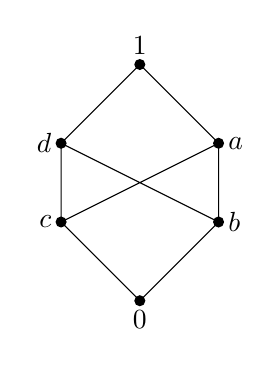
\begin{tikzpicture}
		\fill(0,0)circle(2pt);
		\fill(1,-1)circle(2pt);
		\fill(1,-2)circle(2pt);
		\fill(-1,-1)circle(2pt);
		\fill(-1,-2)circle(2pt);
		\fill(0,-3)circle(2pt);
		\draw(0,0)node[above]{$1$}
			--(1,-1)node[right]{$a$}
			--(1,-2)node[right]{$b$}
			--(0,-3)node[below]{$0$}
			--(-1,-2)node[left]{$c$}
			--(-1,-1)node[left]{$d$}--(0,0)
			(-1,-1)--(1,-2) (1,-1)--(-1,-2);
	\end{tikzpicture}
	\caption{}
	\label{figure:格论.偏序集1}
\end{figure}

\begin{definition}
%@see: 《离散数学》(邓辉文) P155 定义5-19
设\(\opair{L,\leq}\)是偏序集.
若\(L\)中任意两个元素都存在上确界和下确界,
则称\(\opair{L,\leq}\)是\DefineConcept{偏序格}(lattice).
%TODO 缺少定义:偏序集中任意两个元素的上确界、下确界
%@see: https://mathworld.wolfram.com/Lattice.html
\end{definition}

\begin{example}
%@see: 《离散数学》(邓辉文) P155 例5-27
设\(X\)是非空集合.
证明:\(\opair{\Powerset X,\subseteq}\)是偏序格.
\begin{proof}
显然\(\opair{\Powerset X,\subseteq}\)是偏序集.
对于任意\(A,B \in \Powerset X\),有\[
	\sup\{A,B\}
	= A \cup B
	\in \Powerset X,
	\qquad
	\inf\{A,B\}
	= A \cap B
	\in \Powerset X,
\]
所以\(\opair{\Powerset X,\subseteq}\)是偏序格.
\end{proof}
\end{example}

\begin{example}
%@see: 《离散数学》(邓辉文) P155
设\(A,B\)都是非空集合,
\(R\)是\(A\)与\(B\)的笛卡尔乘积\(A \times B\).
证明:\(\opair{R,\subseteq}\)是偏序格.
%TODO proof
% \begin{proof}
% 显然\(\opair{R,\subseteq}\)是偏序集.
% 对于任意\(x,y \in R\),有\[
% 	\sup\{x,y\}
% 	=
% \]
% \end{proof}
\end{example}

\begin{example}
%@see: 《离散数学》(邓辉文) P155 例5-28
设\(D_n\)是正整数\(n\)的全体正因数,即\[
	D_n = \Set{ x\in\mathbb{N}^+ \given x \mid n }.
\]
证明:\(\opair{D_n,\mid}\)是偏序格.
\begin{proof}
显然\(\opair{D_n,\mid}\)是偏序集.
对于任意\(x,y \in D_n\),有\[
	\sup\{x,y\}
	= \lcm{x,y}
	\in D_n,
	\qquad
	\inf\{x,y\}
	= \gcd{x,y}
	\in D_n,
\]
所以\(\opair{D_n,\mid}\)是偏序格.
\end{proof}
\end{example}

\begin{example}
%@see: 《离散数学》(邓辉文) P155 例5-29
设\(F\)是全体合式公式,\(\implies\)是逻辑蕴含关系.
证明:\(\opair{F,\implies}\)是偏序格.
\begin{proof}
显然\(\opair{F,\implies}\)是偏序集.

对于任意\(A,B \in F\),
由于\(A \implies A \lor B,
B \implies A \lor B\),
于是\(A \lor B\)是\(\{A,B\}\)的上界.
如果\(A \implies C,
B \implies C\),
那么\(A \lor B \implies C\),
所以\(\sup\{A,B\}
= A \lor B
\in F\).

对于任意\(A,B \in F\),
因为\(A \land B \implies A,
A \land B \implies B\),
于是\(A \land B\)是\(\{A,B\}\)的下界.
如果\(C \implies A,
C \implies B\),
那么\(C \implies A \land B\),
所以\(\inf\{A,B\}
= A \land B
\in F\).
\end{proof}
\end{example}

\begin{definition}
%@see: 《离散数学》(邓辉文) P156 定义5-20
设\(\opair{L,\leq}\)是偏序格.
对于任意\(x,y \in L\),
定义二元代数运算\begin{gather*}
	x + y \defeq \sup\{x,y\}, \\
	x \cdot y \defeq \inf\{x,y\}.
\end{gather*}
把\(+\)称为\DefineConcept{求上确界运算}.
%@see: https://mathworld.wolfram.com/Join.html
把\(\cdot\)称为\DefineConcept{求下确界运算}.
%@see: https://mathworld.wolfram.com/Meet.html
\end{definition}

\begin{theorem}
%@see: 《离散数学》(邓辉文) P156 定理5-7
设\(\opair{L,\leq}\)是偏序格,
则对于任意\(x,y \in L\)有\begin{gather*}
	x \leq x + y, \\
	y \leq x + y, \\
	x \cdot y \leq x, \\
	x \cdot y \leq y.
\end{gather*}
%TODO proof 下界 <= 下确界 <= 上确界 <= 上界
\end{theorem}

\begin{proposition}
%@see: 《离散数学》(邓辉文) P156
设\(\opair{L,\leq}\)是偏序格,
\(\geq\)是\(\leq\)的逆,
则\(\opair{L,\geq}\)也是偏序格.
\end{proposition}

应该注意到,\(\opair{L,\leq}\)和\(\opair{L,\geq}\)具有对称性,
\(\opair{L,\leq}\)中任意两个元素的上确界
就是相同元素在\(\opair{L,\geq}\)中的下确界,
\(\opair{L,\geq}\)中任意两个元素的下确界
就是相同元素在\(\opair{L,\leq}\)中的上确界,
即\[
	\sup_{\opair{L,\leq}}\{x,y\}
	= \inf_{\opair{L,\geq}}\{x,y\},
	\qquad
	\inf_{\opair{L,\leq}}\{x,y\}
	= \sup_{\opair{L,\geq}}\{x,y\}.
\]
若\(\opair{L,\leq}\)存在最大元素(记为\(1\)),则\(\opair{L,\geq}\)有最小元素(记为\(0\));
若\(\opair{L,\leq}\)存在最小元素\(0\),则\(\opair{L,\geq}\)有最大元素\(1\).

\begin{definition}
%@see: 《离散数学》(邓辉文) P157 定义5-21
对于任意关于偏序格\(\opair{L,\leq}\)的命题,
同时完成以下操作:\begin{itemize}
	\item 将\(\leq\)改为\(\geq\),
	\item 将\(+\)改为\(\cdot\),
	\item 将\(\cdot\)改为\(+\),
	\item 将\(0\)改为\(1\),
	\item 将\(1\)改为\(0\),
\end{itemize}
所得到的命题
称为原命题的\DefineConcept{对偶命题}.
\end{definition}

\begin{theorem}
%@see: 《离散数学》(邓辉文) P157 定理5-8
任意关于偏序格\(\opair{L,\leq}\)的真命题的对偶命题也是真命题.
\end{theorem}

\section{分配格}
一般地,偏序格不满足分配律.

例如,由\hyperref[figure:格论.偏序集2]{钻石格的哈斯图}可知\begin{gather*}
	a \cdot (b + c) = a \cdot 1 = a, \\
	(a \cdot b) + (a \cdot c) = 0 + 0 = 0,
\end{gather*}
从而\(a \cdot (b + c) \neq (a \cdot b) + (a \cdot c)\),
即钻石格的\(\cdot\)运算对\(+\)运算不可分配.

\begin{figure}[hbt]
%@see: 《离散数学》(邓辉文) P155 图5-3(a)
	\centering
	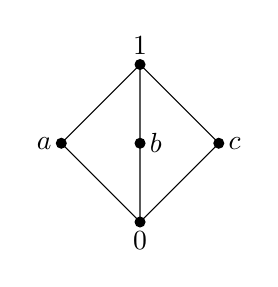
\begin{tikzpicture}
		\fill(0,0)circle(2pt)node[above]{$1$};
		\fill(1,-1)circle(2pt)node[right]{$c$};
		\fill(0,-1)circle(2pt)node[right]{$b$};
		\fill(-1,-1)circle(2pt)node[left]{$a$};
		\fill(0,-2)circle(2pt)node[below]{$0$};
		\draw(0,0)--(1,-1)--(0,-2)--(0,0)--(-1,-1)--(0,-2);
	\end{tikzpicture}
	\caption{钻石格的哈斯图}
	\label{figure:格论.偏序集2}
\end{figure}

类似地,由\hyperref[figure:格论.偏序集3]{五角格的哈斯图}可知,
五角格的\(\cdot\)运算对\(+\)运算不可分配.

\begin{figure}[hbt]
%@see: 《离散数学》(邓辉文) P155 图5-3(b)
	\centering
	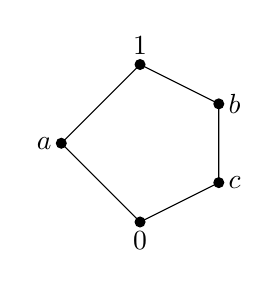
\begin{tikzpicture}
		\fill(0,0)circle(2pt)node[above]{$1$};
		\fill(1,-.5)circle(2pt)node[right]{$b$};
		\fill(1,-1.5)circle(2pt)node[right]{$c$};
		\fill(0,-2)circle(2pt)node[below]{$0$};
		\fill(-1,-1)circle(2pt)node[left]{$a$};
		\draw(0,0)--(1,-.5)--(1,-1.5)--(0,-2)--(-1,-1)--(0,0);
	\end{tikzpicture}
	\caption{五角格的哈斯图}
	\label{figure:格论.偏序集3}
\end{figure}

\begin{definition}
%@see: 《离散数学》(邓辉文) P158 定义5-23
设\(\opair{L,\leq}\)是偏序格.
若\(L\)的\(\cdot\)运算对\(+\)运算可分配,
或\(L\)的\(+\)运算对\(\cdot\)运算可分配,
则称“\(\opair{L,\leq}\)是\DefineConcept{分配格}(distributive lattice)”.
\end{definition}

\section{有补格}
一般来说,偏序格\(L\)不一定存在最大元与最小元.
例如实数集\(\mathbb{R}\)关于小于等于关系\(\leq\)的偏序格\(\opair{R,\leq}\).

\begin{definition}
%@see: 《离散数学》(邓辉文) P159 定义5-24
设\(\opair{L,\leq}\)是偏序格.
若\(L\)存在最大元和最小元,
则称“\(\opair{L,\leq}\)是\DefineConcept{有界格}(bounded lattice)”.
\end{definition}

按偏序集中的约定:
有界格的最大元记为\(1\),最小元记为\(0\).

由定义可知,在有界格\(\opair{L,\leq}\)中,
对任意\(x \in L\),有\(0 \leq x \leq 1\).
进而有\begin{gather*}
	x + 1 = 1, \\
	x \cdot 1 = x, \\
	x + 0 = x, \\
	x \cdot 0 = 0.
\end{gather*}
于是,\(1\)是\(\opair{L,\cdot}\)的单位元,
\(0\)是\(\opair{L,+}\)的单位元.

\begin{example}
%@see: 《离散数学》(邓辉文) P159 例5-33
设\(X\)是非空集合.
证明:\(\opair{\Powerset X,\subseteq}\)是有界格.
%TODO proof
\end{example}

\begin{proposition}
%@see: 《离散数学》(邓辉文) P159
任意有限格是有界格.
%TODO proof
\end{proposition}

\begin{definition}
%@see: 《离散数学》(邓辉文) P159 定义5-25
设\(\opair{L,+,\cdot}\)是有界格,
\(a \in L\).
若存在\(b \in L\)使得\(a + b = 1\)且\(a \cdot b = 0\),
则称“\(b\)是\(a\)的\DefineConcept{补元}”.
\end{definition}

显然,在任意有界格中,若\(b\)是\(a\)的补元,则\(a\)是\(b\)的补元;
\(0\)与\(1\)互为补元;
但是,不是每个元素都有补元,同一个元素的补元未必唯一.

\begin{example}
%@see: 《离散数学》(邓辉文) P159 例5-34
讨论哈斯图 \labelcref{figure:格论.偏序集4} 所示的偏序格中每个元素的补元.
\begin{figure}[hbt]
%@see: 《离散数学》(邓辉文) P159 图5-6
	\centering
	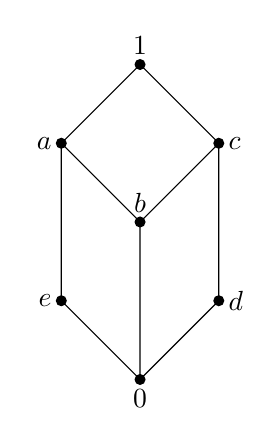
\begin{tikzpicture}
		\fill(0,0)circle(2pt)node[above]{$1$};
		\fill(1,-1)circle(2pt)node[right]{$c$};
		\fill(1,-3)circle(2pt)node[right]{$d$};
		\fill(0,-4)circle(2pt)node[below]{$0$};
		\fill(-1,-3)circle(2pt)node[left]{$e$};
		\fill(-1,-1)circle(2pt)node[left]{$a$};
		\fill(0,-2)circle(2pt)node[above]{$b$};
		\draw(0,0)--(1,-1)--(1,-3)--(0,-4)--(-1,-3)--(-1,-1)--(0,-2)
			(0,0)--(-1,-1) (0,-4)--(0,-2)--(1,-1);
	\end{tikzpicture}
	\caption{}
	\label{figure:格论.偏序集4}
\end{figure}
\begin{solution}
\(0\)与\(1\)互为补元.
\(a\)的补元是\(d\).
\(b\)的补元不存在.
\(c\)的补元是\(e\).
\(d\)的补元是\(a\)和\(e\).
\(e\)的补元是\(c\)和\(d\).
\end{solution}
\end{example}

